\chapter{Software Design, State Of The Art} \label{chapter3}
\minitoc
\eject

\cit{A designer is responsible for producing the greatest benefit for any given investment of time, talent, money, and other resources.}{K. Sullivan, W. Griswold, Y. Cai, B. Hallen \cite{Sullivan2001}}

With the growth of Software as a Service (SaaS) on the web, the same company carries both development and exploitation of an application at scale of unprecedented size.
It revealed the importance of previously unknown economic constraints.
To assure the continuous growth and sustainability of an application, it needs to address two contradictory goals : development productivity and performance efficiency.
These goals needs to be enforced by the platform supporting the application to build good development habits for the developers.
A platform designates any solution that allows to build an application on top of it, including programming languages, compilers, interpreters, frameworks, runtime libraries and so on.

The productivity of a platform is the degree to which developers can quickly produce new and modify existing softwares.
It impacts the maintainability of the applications and relies on the modularity enforced by its platform.
\textit{75\% of your budget is dedicated to software maintenance.}\ftnt{http://www.castsoftware.com/glossary/software-maintainability}
Especially, higher order programming is crucial to build and compose modules productively.
It relies either on mutable states, or immutable states, but hardly on a combination of both.

However, neither mutable nor immutable states allows performance efficiency.
Mutable states leads to synchronization overhead at a coarser-grain level, while immutable states leads to communication overhead at a finer-grain level.
Efficiency relies on a combination of synchronization at a fine-grain level, and immutable message passing at a coarse-grain level.
This combination breaks the modularity, hence the productivity of an application.
A company has no choice but to commit huge development efforts to get efficient performances.

\illustration{virtuous circle between community and industry}
Moreover, a balance between productivity and efficiency is required for a platform to enter a virtuous circle of adoption.
The productivity is required to be appealing to gather a community to support the ecosystem around the platform.
This community is appealing for the industry as a hiring pool.
Additionally, the efficiency is required to be adopted by the industry to be economically viable.
And the industrial relevance provides the reason for this ecosystem to exist and the community to gather.

This chapter presents a broad view of the state of the art in the compromises between productivity and efficiency.
It defines software productivity, efficiency, and adoption in section \ref{chapter3:definitions} and all the underlying concepts, such as higher order programming and state mutability.
It then analyzes different platforms according to their focus. platforms focusing on productivity are addressed in section \ref{chapter3:software-productivity}, those focusing on efficiency in section \ref{chapter3:software-efficiency} and those focusing on a compromise between the two in section \ref{chapter3:software-adoption}.

\section{Definitions} \label{chapter3:definitions}

The continuous growth and sustainability offered by a platform relies on three criteria.
This section defines these tree criteria, as well as all the underlying concepts.

Additionally, for the context of this thesis, a fourth criterium appears in this list.
It is important for the analyzed platforms to be web compliant.\nt{I don't know where to put this criterium}

\begin{itemize}
\item Maintainability
\item Performance Efficiency
\item Adoption
\item Web compliance
\end{itemize}

\subsection{Maintainability}

Software maintainability is defined as the degree to which an application can be understood, fixed, and extended.
% For an application to be maintainable, it needs to be modular.
%Maintainability relies on modularity.
For an application to be maintainable, its frameworks need to enforce modularity directly in the design.
% It relies on two factors, module encapsulation and module composition.

\subsubsection{Modularity}

The modularity of a software implementation is about encapsulating subproblems and composing them to allow greater design to emerge.
It allows to limit the understanding required to contribute to a module \cite{Stevens1974}, which helps developers to repair and enhance the application. 
Additionally, it reduces development time by allowing several developers to simultaneously implement different modules \cite{Wong2009,Cataldo2006}.

The criteria to define modules to improve maintainability are low coupling and high cohesion \cite{Stevens1974}.
Coupling defines the strength of the interdependence between modules.
Cohesion defines how strongly the features inside a module are related.
% Encapsulating a subproblem into a module helps increase cohesion.
% Composition abstractions helps decrease their coupling.
The composition of modules help decrease coupling, and encapsulation helps increase their cohesion.
Encapsulation and composition improves maintainability.

\begin{itemize}
\item Encapsulation $\to$ High Cohesion
\item Composition $\to$ Low Coupling
\end{itemize}

\subsubsection{Encapsulation}

\paragraph{Boundary Definition}

\illustration{spaghetti programming}
Modular Programming stands upon Structured Programming \cite{Dijkstra1970}.
% Dijkstra firstly developed the concept of Structured Programming \cite{Dijkstra1970}, which later led to modular programming.
% It is defined as \textit{the systematic use of abstraction to control a mass of details, and also a means of documentation which aids program design} \cite{Knuth1974}.
It draws clear interfaces around a piece of implementation so that the execution is enclosed inside.
At a fine level, it helps avoid spaghetti code \cite{Dijkstra1968a}, and at a coarser level, it structures the implementation \cite{Dijkstra1968} into modules, or layers.
% The next paragraph explains further the criteria to draw the borders around modules.

\paragraph{Data Protection}

\illustration{lasagna programming}
Modular programming encapsulates a specific design choice in each module, so that it is responsible for one and only one concern.
It isolates its evolution from impacting the rest of the implementation \cite{Parnas1972, Tarr1999, Hursch1995}.
Examples of such separation of concerns are the separation of the form and the content in HTML / CSS, or the OSI model for the network stack.

\subsubsection{Composition} \label{chapter3:software-maintainability:modularity:features}

\paragraph{Higher-Order Programming}
\nt{If possible, include this reference : Continuations and coroutines \cite{Haynes1984}}

Higher-order programming allows to manipulate functions like any other primary value : to store them in variables, or to pass them as arguments.
It replaces the need for most modern object oriented programming design patterns \ftnt{http://stackoverflow.com/a/5797892/933670} with Inversion of Control \cite{Johnson}, the Hollywood Principle \cite{Sweet1985}, and Monads \cite{Wadler1992}.
Higher-order programming help loosen coupling, thus improve maintainability.

In languages allowing mutable state, higher-order functions are implemented as closure, to preserve the lexical scope \cite{Sussman1998}.
A closure is the association of a function and a reference to the lexical context from its creation.
It allows this function to access variable from this context, even when invoked outside the scope of this context.
\nt{next sentence is redundant with the suit}
It eventually tangles the memory references so that it requires a global memory.

\paragraph{Lazy Evaluation}

Lazy evaluation is an evaluation strategy allowing to defer the execution of a function only when its result is needed.
% And according to \cite{Hughes1989}, \textit{Abelson and Sussman stress that streams (lazy list) is a powerful tool for structuring programs \cite{Sussman1983}.
The lazy evaluation of lists is equivalent to a stream with a null-sized buffer, while the opposite, eager evaluation, corresponds to an infinite buffer \cite{VanRoy2003}.
\nt{find another transition}Indeed, the dataflow programming paradigm resulting from lazy lists is particularly adapted for stream processing applications.

\nt{This paragraph is not very clear}
The lazy evaluation, as well as streams are powerful tools for structuring modular programs \cite{Sussman1983}.
Lazy evaluation allows the execution to be organized as a concurrent pipeline, as the stages are executed independently for each element of the stream.
But this concurrency requires immutability of state, or at least isolation of side-effects.\nt{why ? explain or point to the explanation}
The next section addresses the consequences of higher-order programming and lazy evaluation on parallelism.



\paragraph{}

The criteria to analyze platform for maintainability are the following.

\begin{itemize}
\item Encapsulation $\to$ High Cohesion
  \subitem Boundary definition
  \subitem Data protection
\item Composition $\to$ Low Coupling
  \subitem Higher-order programming, Lambda Expressions
  \subitem Lazy evaluation, Stream composition
\end{itemize}


\subsection{Performance Efficiency}

The performance efficiency of a software project is the relation between the usage made of available resources and the delivered performance.
For an application to perform efficiently, the frameworks used need to enforce scalability directly in its design.

Scalability relies on the commutativity of operations execution \cite{Clements2013a}.
Operations are commutative if the order of their executions is irrelevant for the correctness of their results.
Commutativity assures the independence of operations.

\subsubsection{Independence}

The independence, and commutativity of an operations depends on its accesses to shared state.
If the operations doesn't rely on any shared state, it is independent.
The independence of operations allows to execute them in parallel, hence to increase performance proportionally to occupied resources \cite{Amdahl1967,Gunther1993}.
But if they rely on shared state, they need to coordinate their timing of execution to avoid conflicting accesses.
This coordination can be done in two ways.
\begin{description}
\item[Synchronization] Operations are scheduled sequentially to have an exclusive access to a centralized state, or
\item[Message-passing] Operations communicate their local modifications of the state to other operations, in a decentralized fashion.
\end{description}

If the operations access the state too frequently, the communication overhead exceed the performance gains of parallelism.
And if operations access the state too rarely, the centralization of the state limits the parallelism.
Operations tend to share state closely at a fine-grain level and less at a coarser-grain level.
% Therefore, at a fine-grain level the operations need to be scheduled sequentially to avoid the communication overhead.
% And at a coarse-grain level they need to communicate via message-passing, to allow parallelism.
Therefore, performance efficiency requires the combination of fine-level state sharing to avoid communication overhead, and coarse-level independence to allow parallelization \cite{Gustafson1988,Gunther1996,Nelson1996,Gunther2002}.

\paragraph{}

The criteria to analyze platform for their performance are the following.

\begin{itemize}
\item Fine-level state sharing
  \subitem State mutability $\to$ Synchronization
\item Coarse-level independence
  \subitem State immutability $\to$ Message-passing
\end{itemize}

\nt{Is it the right place to put that ?}
The threshold determining frequent or rare access to the state determines the granularity level between synchronization and parallelization of tasks.
This granularity needs to be free from the decomposition into modules.
If the too are related, they interfere with each other, and impact either maintainability, or performance.


\subsubsection{Asynchronism}
TODO ?


\subsubsection{Atomicity}
TODO ?



% \subsubsection{Event-Loop Execution Model} \label{chapter2:web-as-a-platform:javascript:event-loop}

% \nt{Reduce the event-loop explanation to the bare minimum, the definitions of callbacks and promises should be in the state of the art. It only need to present briefly how the event-loop works to understand the problem}

% Javascript is often associated with an event-based paradigm to react to concurrent user interactions.
% In 2009, Joyent released Node.js to build real-time web services with this paradigm.
% It is a server-side implementation of Javascript based on an event-loop.
% This event-based paradigm proved to be very efficient as well for a web service to react to concurrent requests.
% This section presents the event-loop execution model, and the advantages of Javascript for this paradigm.

% The event-loop efficiency comes from non-blocking communications, asynchronous execution, and cooperative scheduling.
% It relies on a queue storing the messages received asynchronously.
% The loop executes tasks previously defined to process these messages one after the other.
% Each task can initiate new communications, leading in turn to the queuing of more messages, which trigger more tasks, and so on.
% Each task is executed atomically and exclusively, until it yields execution to continue with the next task in queue.

% \nt{TODO schema of an event-loop}

% \paragraph{Callbacks}

% In Javascript, the asynchronous communications are initiated by function calls.
% The callee immediately returns to avoid the caller to wait for the result.
% The task to process the result of the communication, and to continue the execution afterward, is a function passed as an argument to the callee.
% This function is named a callback or a continuation.
% A callback is a function passed as an argument to a callee.
% It is a continuation if the callee calls it to transfer the control back to the caller without the need for synchronization.

% In this execution model, the control flow follows the asynchronous function calls and callbacks.
% It organizes the execution of callbacks causally, one after the other, similarly to a pipeline.
% Indeed, the input stream of data flows through a sequence of callbacks until the application outputs it.
% In this model, callbacks are the atoms of the asynchronous execution flow control.
% The next paragraph presents a more elaborate form of control.

% \paragraph{Promises}

% Since the asynchronous execution flow became more complicated on larger web application, many projects proposed improved asynchronous execution controls on top of callbacks.
% The ECMAScript specification proposes Promises for such purpose.
% It arranges sequences of causally related callbacks into cleanly organized pipelines of callbacks communicating their results to the next.

% \paragraph{Closures}

% Because callbacks can be passed as an argument, they are first class citizen and imply higher-order programming. %, which is part of functional programming.
% % Javascript features higher-order functions.
% For a callback to continue the execution without needing synchronization with the caller, it needs to have access to the initial context of the caller.
% This context is linked with the function when passed to the callee.
% The association of a function and its initial context is called a closure.

% Higher-order programming is convenient for developers, as they allow great modularity in the implementation through \textit{e.g.} inversion of control.
% It is presented in further details in section \ref{chapter3:software-maintainability}.
% However, because the contexts are passed, and shared all over the implementation, this programming model needs a global memory for coordination.
% A global memory is problematic to increase the concurrency of the execution.

% This section presented Javascript as the language of the web, and its programming model.
% The next section presents the realities and technical challenges to assure the performance of web services against billions of users.






\subsection{Adoption}

An application is sustainable only if the frameworks used to build it generate reinforcing interactions between a community of passionate and the industry.
A framework needs to present a balance between maintainability and performance efficiency to be adopted by both the community and the industry.
The maintainability is required for a framework to be appealing to gather a community to support the ecosystem around it.
And the performance efficiency is required to be economically viable and needed by the industry, and to provide the reason for this ecosystem to exist.

\begin{itemize}
\item Community Support
\item Industrial Need
\end{itemize}

\paragraph{}

This incentive to balance between maintainability and performance efficiency is illsutrated in figure \ref{fig:state-of-the-art}.

\begin{figure}[h!] \label{fig:state-of-the-art}
\begin{center}
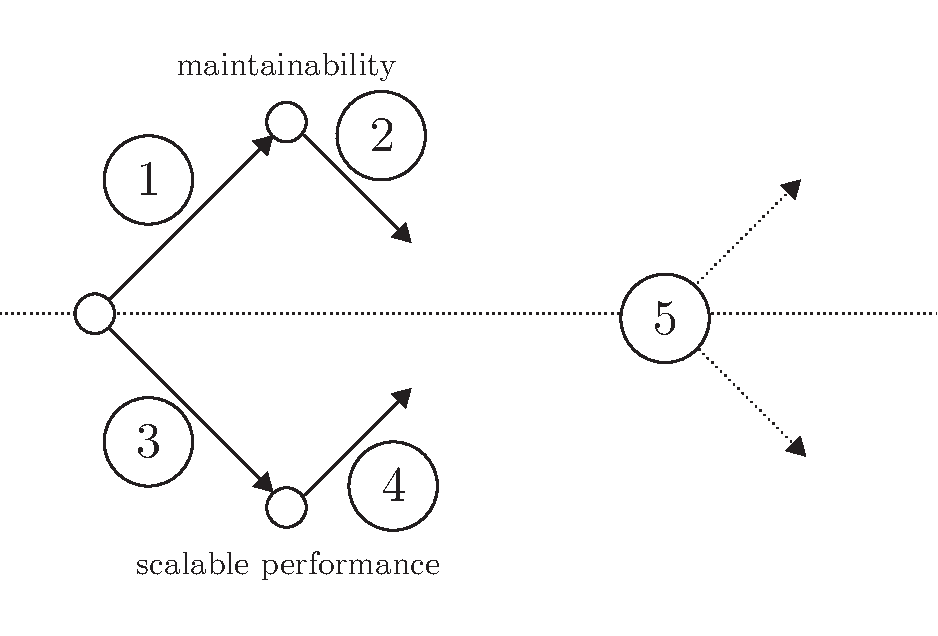
\includegraphics[width=0.6\textwidth]{../ressources/state-of-the-art.pdf}
\end{center}
\end{figure}


\subsection{Web}

Pour la justification Web, je pense que tu dois raisonner que c'est le seul marché réellement explosif, donc c'est celui que tu vises. 

Il y a pas mal d'arguments pour cibler le web :
- technologies assez peu connues, car souvent imaginées comme n'étant qu'un problème d'ihm,
- omniprésence sur internet,
- et comme tout business doit passer par Internet, il faut comprendre le web en priorité. 

Ne bloque pas trop sur le Web, pour moi c'est le contexte de fond, donc il faut que les plateformes soient orientées web. Je pense qu'un autre argument lié au web, c'est celui de TCP/IP, c'est à dire que les plateformes doivent accepter le délais dans les échanges. 
\section{Productivity Focused Platforms} \label{chapter3:software-productivity}

\cit{It is becoming increasingly important to the data-processing industry to be able to produce
[programming systems] % more programming systems and produce them with fewer errors,
at a faster rate, and in a way that modifications can be accomplished easily and quickly.}{W. Stevens, G. Myers, L. Constantine \cite{Stevens1974}.}

\nt{TODO read Sackman, Erickson, Grant 1968 about the 10x in productivity %
http://dl.acm.org/citation.cfm?id=362858 %
All programmers had at least 7 years experience %
Range of initial coding times 20:1 %
Range of debugging times 25:1 %
Range of program sizes produced 5:1 %
Range of program execution speeds 10:1 %
 %
Enormous variation in individual and team productivity, compared to variation in method productivity. %
 %
Last measurement Boehm 2000 5.3:1 for team productivity %
}

In order to improve and maintain a software system, it is important to holds in mind a mental representation of its implementation.
As the system grows in size, the mental representation becomes more and more difficult to grasp.
Therefore, it is crucial to decompose the system into smaller subsystem easier to grasp individually.
% This section presents academic propositions for software productivity, and then presents how the industry adapted these solutions to meet their needs.
% Finally, this section presents the limitations of the presented solutions.

% \nt{Interesting, but to be rewritten: 
% Architects, and mechanical engineers draw codified plans to share their mental representations with peers and building teams.
% software design is an exception in that the implementation is both the shared mental representation, and the actual product.
% The mental representation is often lost in technical details and optimizations for the actual product.
% }

\cit{Measuring programming progress by lines of code is like measuring aircraft building progress by weight.}{Bill Gates}

Section \ref{chapter3:software-productivity:modularity} presents the modular programming paradigms, and their programming models, oriented toward productivity.
Section \ref{chapter3:software-productivity:adoption} presents the adoption of the implementations of modular programming languages.
Section \ref{chapter3:software-productivity:performance-limitations} presents the consequences of the modularity on performance.
Finally, section \ref{chapter3:software-productivity:summary} summarizes the three previous sections in a table.

\subsection{Modular Programming} \label{chapter3:software-productivity:modularity}

\begin{figure}[!h]
\begin{center}
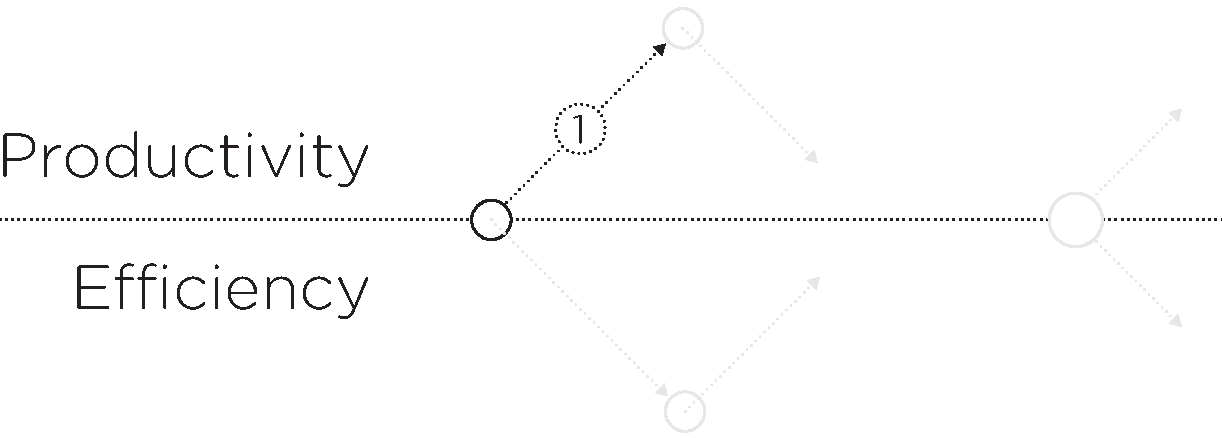
\includegraphics[width=0.6\textwidth]{../resources/state-of-the-art-1.pdf}
\end{center}
\caption{Focus on Productivity}
\label{fig:state-of-the-art-1}
\end{figure}

% The modularity of a software implementation is about enclosing subproblems and composing them through relevant interface abstractions.
% % It allows greater design to emerge from the composition of smaller components.
% It improves the productivity of an implementation, as illustrated in figure \ref{fig:modular-programming-state-of-the-art}.
% It allows to limit the understanding required to contribute to a module \cite{Stevens1974}.
% And it reduces development time by allowing several developers to simultaneously implement different modules \cite{Wong2009,Cataldo2006}.

% % \nt{Read and include \cite{Simon1962}}

% % \subsubsection{Design Choices} \label{chapter3:software-productivity:design-choices}

% % \nt{TODO this introduction is not very clear}
% % In the decomposition of a large problem into smaller subproblem, there is two design choices.
% % The first one is the granularity, and organization of the subproblems within the system decomposition.
% % The second one is the organization of the implementation within the subproblems to improve productivity.

% % \nt{reduce all these paragraph into a concise one and move it into the introduction}

% % \paragraph{System Decomposition}

% \illustration{spaghetti programming}
% Modular Programming stands upon Structured Programming \cite{Dijkstra1970}.
% % Dijkstra firstly developed the concept of Structured Programming \cite{Dijkstra1970}, which later led to modular programming.
% % It is defined as \textit{the systematic use of abstraction to control a mass of details, and also a means of documentation which aids program design} \cite{Knuth1974}.
% It draws clear interfaces around a piece of implementation so that the execution is enclosed inside.
% At a fine level, it helps avoid spaghetti code \cite{Dijkstra1968a}, and at a coarser level, it structures the implementation \cite{Dijkstra1968} into modules, or layers.
% % The next paragraph explains further the criteria to draw the borders around modules.
% \illustration{lasagna programming}
% Encapsulate a specific design choice in each module, so that it is responsible for one and only one concern, isolate its evolution from impacting the rest of the implementation \cite{Parnas1972, Tarr1999, Hursch1995}.
% Examples of such separation of concerns are the separation of the form and the content in HTML / CSS, or the OSI model for the network stack.

% The criteria to define modules to improve productivity are coupling and cohesion \cite{Stevens1974}.
% The coupling defines the strength of the interdependence between modules, while cohesion defines how strongly the features inside a module are related.
% Low coupling between modules and high cohesion inside modules helps logically organize, and understand the implementation.
% Hence, it improve its productivity.

% The composition of modules with low coupling is provided by encapsulation, higher-order programming and lazy evaluation.
% Hence, the criteria to analyze the solutions presented in this section regarding productivity are :
% \begin{itemize}
% \item encapsulation mechanism
% \item presence of higher-order programming
% \item presence of lazy evaluation, or stream composition
% \end{itemize}
% The last two criteria provide composition abstractions to design solutions from smaller components.
% Encapsulation and composition are the features in modular programming that produce productivity.

% The next paragraphs present the last two criteria \ref{chapter3:software-productivity:modularity:features}, and  then the main programming models, section \ref{chapter3:software-productivity:modularity:programming-models}.

% \paragraph{Decomposition Criteria}

% \nt{move this paragraph closer to OOP ?}
% The criteria to define modules to improve productivity are coupling and cohesion \cite{Stevens1974}.
% The coupling defines the strength of the interdependence between modules, while cohesion defines how strongly the features inside a module are related.
% Low coupling between modules and high cohesion inside modules helps logically organize, and understand the implementation.
% Hence, it improve its productivity.
% The next paragraph presents the approach to build modules helping with the evolution of the implementation.

% \paragraph{Development Evolution}

% \nt{productivity also relies on supporting implementation evolution}

% The modular organization should isolate the evolution of a module from impacting the rest of the implementation.
% Encapsulate a specific design choice in each module, so that it is responsible for one and only one concern, isolate its evolution from impacting the rest of the implementation \cite{Parnas1972, Tarr1999, Hursch1995}.
% Examples of separation of concerns are the separation of the form and the content in HTML / CSS, or the OSI model for the network stack.
% The information hiding principle advocates to encapsulate a specific design choice in each module.
% The Separation of Concerns advocates each module to be responsible for one and only one specific concern.

% Figure \ref{fig:modular-programming-state-of-the-art} illustrates an overview of the direction of modular programming regarding the general trends in software design.
% Section \ref{chapter3:software-productivity:design-choices} presents the decomposition.

% \subsubsection{Programming Models} \label{chapter3:software-productivity:programming-models}

% \subsubsection{Features} \label{chapter3:software-productivity:modularity:features}

% \paragraph{Higher-Order Programming}
% \nt{If possible, include this reference : Continuations and coroutines \cite{Haynes1984}}

% Higher-order programming allows to manipulate functions like any other primary value : to store them in variables, or to pass them as arguments.
% It replaces the need for most modern object oriented programming design patterns \ftnt{http://stackoverflow.com/a/5797892/933670} with Inversion of Control \cite{Johnson}, the Hollywood Principle \cite{Sweet1985}, and Monads \cite{Wadler1992}.
% Higher-order programming help loosen coupling, thus improve productivity.

% In languages allowing mutable state, higher-order functions are implemented as closure, to preserve the lexical scope \cite{Sussman1998}.
% A closure is the association of a function and a reference to the lexical context from its creation.
% It allows this function to access variable from this context, even when invoked outside the scope of this context.
% \nt{next sentence is redundant with the suit}
% It eventually tangles the memory references so that it requires a global memory.

% \paragraph{Lazy Evaluation}

% Lazy evaluation is an evaluation strategy allowing to defer the execution of a function only when its result is needed.
% % And according to \cite{Hughes1989}, \textit{Abelson and Sussman stress that streams (lazy list) is a powerful tool for structuring programs \cite{Sussman1983}.
% The lazy evaluation of lists is equivalent to a stream with a null-sized buffer, while the opposite, eager evaluation, corresponds to an infinite buffer \cite{VanRoy2003}.
% \nt{find another transition}Indeed, the dataflow programming paradigm resulting from lazy lists is particularly adapted for stream processing applications.

% \nt{This paragraph is not very clear}
% The lazy evaluation, as well as streams are powerful tools for structuring modular programs \cite{Sussman1983}.
% Lazy evaluation allows the execution to be organized as a concurrent pipeline, as the stages are executed independently for each element of the stream.
% But this concurrency requires immutability of state, or at least isolation of side-effects.\nt{why ? explain or point to the explanation}
% The next section addresses the consequences of higher-order programming and lazy evaluation on parallelism.


% \subsubsection{Programming Models} \label{chapter3:software-productivity:modularity:programming-models}

The next paragraphs presents the different programming model regarding their support to modular programming and productivity.
% They represent the number \circled{1} in figure \ref{fig:modular-programming-state-of-the-art}.

\subsubsection{Imperative Programming}

Imperative programming is the very first programming paradigm, as it evolves directly from the hardware architectures.
It allows to express the suite of operation to carry sequentially on the computing processor.
% Lots of programming languages feature imperative programming.
Most imperative languages provide encapsulation with modules but not higher-order programming, nor lazy evaluation.
The implementations of Imperative Programming 

\subsubsection{Object Oriented Programming}

\illustration{multiple cells communicating}

% Alan Kay, who coined the term, states that Object Oriented Programming (OOP) is about message-passing, encapsulation and late binding.
% (There is no academic reference for that, only a public mail exchange\ftnt{http://userpage.fu-berlin.de/~ram/pub/pub\_jf47ht81Ht/doc\_kay\_oop\_en}.)
% Message-passing and late binding loosen coupling between objects, while encapsulation is intended to increase cohesion \ftnt{http://williamdurand.fr/2013/06/03/object-calisthenics/}.
% % Reducing coupling and increasing cohesion are further sought by object calisthenics, in the chapter 6 of \textit{The Thoughtworks Anthology} \cite{Bay2008}

The very first Object-Oriented Programming (OOP) language was Smalltalk \cite{Goldberg1984}.
It defined the core concepts as message passing and encapsulation %, and dynamic binding
\ftnt{http://userpage.fu-berlin.de/~ram/pub/pub\_jf47ht81Ht/doc\_kay\_oop\_en}.
Nowadays, the emblematic figures in the software industry are C++ \ImplementationsOf{Object-Oriented Programming}.
% Though, the trend seems to digress from these languages to evolve toward a more dynamic approach.
% Indeed Javascript adopts some functional features such as dynamic typing and higher-order functions \cite{Ecma1999}.}
They provide encapsulation with Classes, and allows passing mutable structures for performance reasons.
They recently introduced higher-order programming with lambda expressions.

\subsubsection{Functional Programming} \label{chapter3:software-productivity:programming-models:functional-programming}

% \cit{All problems in computer science can be solved by another level of indirection}{Butler Lampson}

The definition of pure Functional Programming resides in manipulating only expressions and forbidding state mutability, replaced by message passing.
The absence of state mutability makes a function side-effect free, hence their execution can be scheduled in parallel.
But it implies heavy message passing, which negatively impact performances.
The most important pure Functional Programming languages are \ImplementationsOf{Functional Programming}.
They provide encapsulation, higher-order programming and lazy evaluation.

\subsubsection{Multi-Paradigm}

The functional programming concepts are also implemented in other languages along with mutable states and object-oriented concepts.
% The two main references of Object-Oriented Programming, Java and C++, adopted higher-order functions in their last version, Java 8 and C++11.
Major recent programming languages, including Java 8 and C++ 11, now commonly present \textbf{higher-order functions} and \textbf{lazy evaluation}. % to help loosen the couple between modules. %, define more generic and reusable modules.
% Moreover, they provide reflective programming, and other meta-programming techniques.
\textit{In fine}, it helps developers to write applications that are more maintainable, and favorable to evolution \cite{Hughes1989,Turner1981}.
These recent multi-paradigms languages such as \ImplementationsOf{Multi Paradigm} combine the different paradigms to help developer building applications faster.
% They provide encapsulation, higher-order programming and stream composition.

\separator

Table \ref{tab:productivity-modularity} presents a summary of the analysis of the programming models presented in the previous paragraphs.

\ModularProductivityTable{tab:productivity-modularity}

% \begin{table}[h!]
% \small
% \begin{tabu} to \linewidth {@{} l X[l] c c c c @{}}
% %
% % \multicolumn{3}{c}{}  & \lab{Concurrency} & \multicolumn{2}{|c}{Parallelism} \\
% Model & Implementations    & \lab{Composition} & \lab{Encapsulation} & $\to$ & \lab{Productivity} \\
% \tabucline[.5pt]{-}%
% Imperative Programming         & C                                             & \X & \V && \X \\ \tabucline[on .5pt]{-}
% Object-Oriented Programming    & C++, Java                                     & \V & \V && \V \\ \tabucline[on .5pt]{-}
% Functional Programming         & Scheme, Miranda, Haskell                      & \V & \V && \V \\ \tabucline[on .5pt]{-}
% Multi Paradigm                 & Javacript, Python, Ruby, Go                   & \V & \V && \V \\
% \tabucline[.5pt]{-}
% \end{tabu}
% \caption{Analysis of the state of the art in modular programming regarding productivity}
% \label{tab:productivity-modularity}
% \end{table}

\subsection{Adoption} \label{chapter3:software-productivity:adoption}

\begin{figure}[!h]
\begin{center}
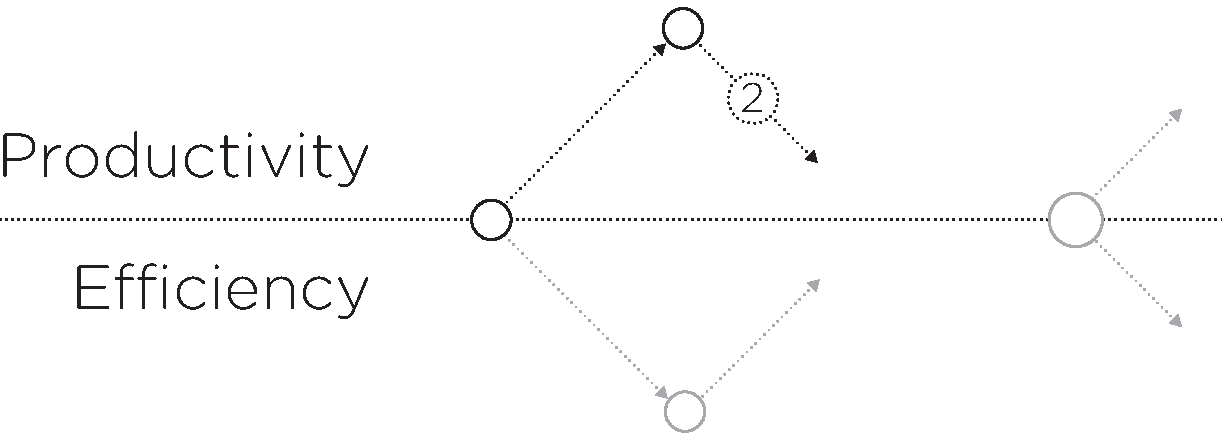
\includegraphics[width=0.6\textwidth]{../resources/state-of-the-art-2.pdf}
\end{center}
\caption{Steering back toward Performence Efficiency}
\label{fig:state-of-the-art-2}
\end{figure}

% A system is maintainable only if there is people willing to maintain it.
% For people to widely adopt a programming language, it needs to be features a balance between performance and productivity.
% It forces the modular programming models to be implemented taking into account not only productivity, but performance as well.
% The balance is steered back toward performance, as illustrated in figure \ref{fig:state-of-the-art-2}.

% Indeed, the immutability of pure functional programming impact performance too negatively to be wildly used in industrial context.
% And the pure object-oriented programming lacks composition abstractions, like higher-order programming and lazy evaluation.
% As a result, the multi-paradigm scripts tends to be better compromises between modularity and performance.
% And the data of this section proves it.

% The criteria to analyze the solutions presented in this section regarding the adoption are the adoption in :
% \begin{itemize}
% \item the community,
% \item the industry,
% \item web technologies
% \end{itemize}
% The first two criteria make sure that the technology is growing organically with a passionate community, and backed by industrial needs.
% The last criteria assures the fitting of the technologies with our economical context of a web application.
The next paragraphs presents the adoption of Javascript, and the other implementations of the presented programming model.
% ->_>_>_>_> These implementations steer back from productivity into performance efficiency, as shown by \circled{2} in figure \ref{fig:modular-programming-state-of-the-art-2}.

% The rise of Javascript is indisputable on the web, and seems to be rising in the software industry as well.
% But it is difficult to give an accurate representation of the situation because the software industry often maintains a fog of war to try to keep an edge.
% The following paragraphs report some efforts to clear up the situation.
% More detailed informations are available section \ref{appendix:langpop}.

\subsubsection{Community}

\paragraph{Available Resources}

As of December 2015, Javascript ranks 8th according to the TIOBE Programming Community index, and was the most rising language in 2014.
This index measure the popularity of a programming language with the number of results on many search engines.
% However, this measure is controversial as the number of pages doesn't represent the number of readers.
And it ranks 7th on the PYPL.
The PYPL index is based on Google trends to measure the number of requests on a programming language.
% However, it is limited to Google searches.

From these indexes, the major programming languages are Java, C++, C, C\# and Python.
% The preponderance of Object-Oriented Languages in these results is explained by the lag of these indexes.
% Java and C/C++ were very popular and helped bring the explosion of the web.
These languages are still widely used by their communities and in the industry.
% Though, the next paragraphs bring a more actual vision.

\nt{TODO graphical ranking of TIOBE and PYPL}

\begin{figure}
  \centering
  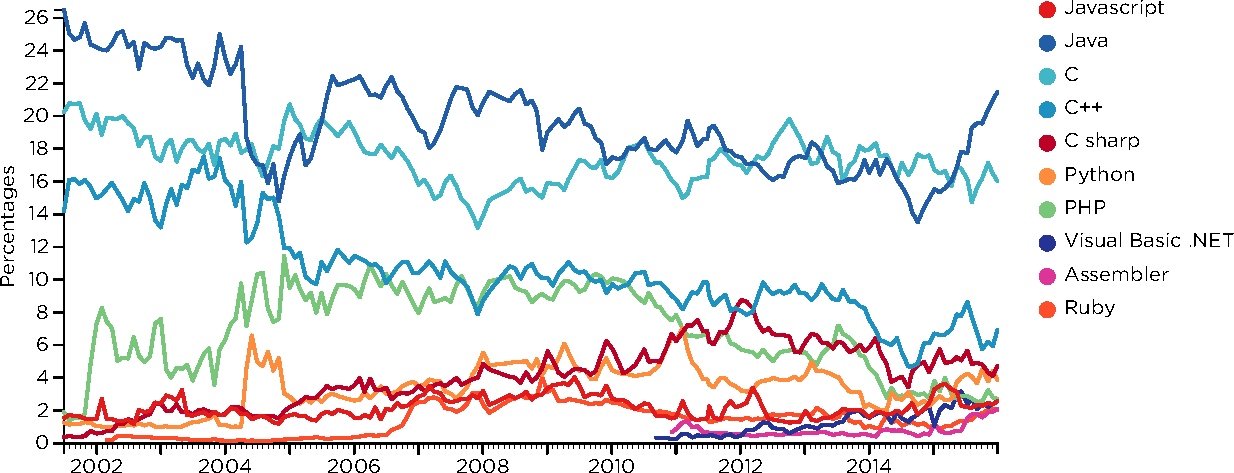
\includegraphics[width=\linewidth]{../resources/tiobe.pdf}
  \label{fig:tiobe}
  \caption{TIOBE ranking}
\end{figure}

\paragraph{Developers Collaboration Platforms}

Online collaboration tools give an indicator of the number of developers and projects using certain languages.
Javascript is the most used language on \textit{Github}\ftnt{the most important collaborative development platform gathering about 9 millions users.} and the most cited language on \textit{StackOverflow}\ftnt{the most important Q\&A platform for developers.}.
It represents more than \num{320000} repositories on \textit{Github}.
The second language is Java with more than \num{220000} repositories.
It is cited in more than \num{960000} questions on \textit{StackOverflow} while the second is Java with around \num{940000} questions.
% According to \textit{Black Duck Software}\ftnt{https://www.blackducksoftware.com/} it is the second language used in open source projects.
% C is first, C++ third and Java fourth.\ftnt{https://www.blackducksoftware.com/resources/data}
% These four languages represent about 80\% of all programming language usage in open source communities.
And according to a survey by \textit{StackOverflow}, it is currently the language the most popular\ftnt{http://stackoverflow.com/research/developer-survey-2015}.
Moreover, the Javascript package manager, \textit{npm}, has the most important and impressive package repository growth.

\nt{TODO include so survey graph}


\begin{figure}
  \centering
  \begin{minipage}{0.49\textwidth}
    \centering
    
\includegraphics[width=\linewidth]{../resources/blackduck-alltime.pdf}
    \label{fig:blackduck-alltime}
    \caption{Blackduck analysis total}
  \end{minipage}
  \hfill
  \begin{minipage}{0.49\textwidth}
    \centering
    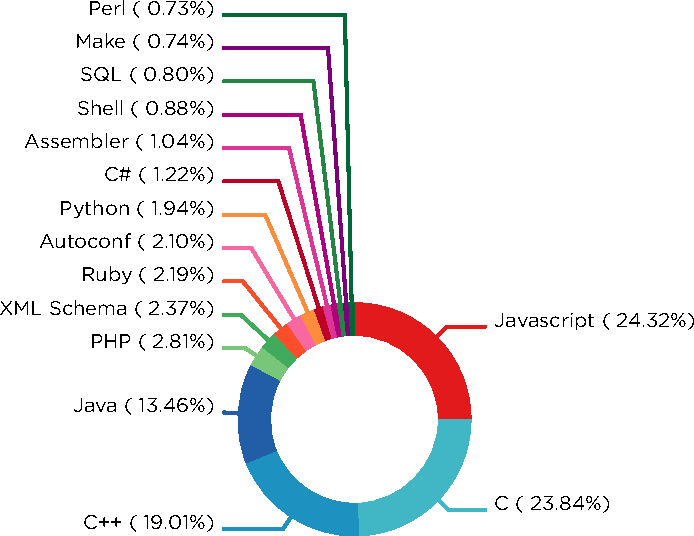
\includegraphics[width=\linewidth]{../resources/blackduck-2015.pdf}
    \label{fig:blackduck-2015}
    \caption{Blackduck analysis for 2015}
  \end{minipage}
\end{figure}


\begin{figure}
  \centering
  
\includegraphics[width=0.7\linewidth]{../resources/stackoverflow-mostwanted.pdf}
  \label{fig:so-tags}
  \caption{Most Wanted Technologies in 2015}
\end{figure}

% \begin{figure}[!h]
%   \begin{floatrow}
%     \ffigbox{
%        
\includegraphics[width=0.9\linewidth]{../resources/blackduck-alltime.pdf}
%     }{
%       \label{fig:blackduck-alltime}
%       \caption{Blackduck analysis total}
%     }
%     \ffigbox{
%        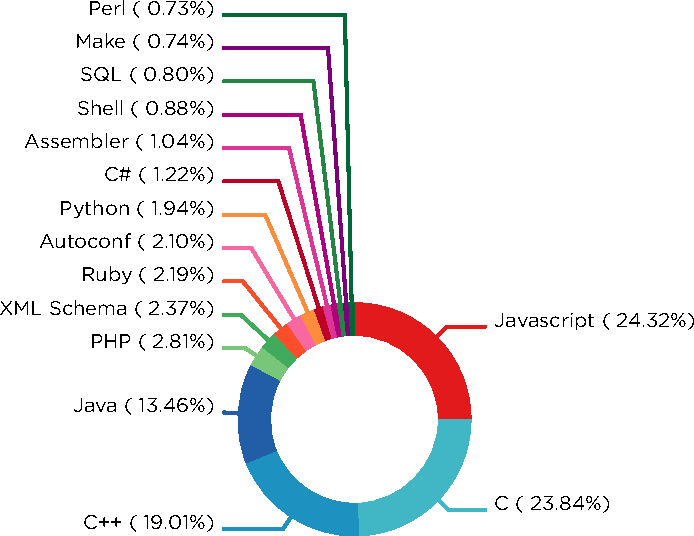
\includegraphics[width=0.9\linewidth]{../resources/blackduck-2015.pdf}
%     }{
%       \label{fig:blackduck-2015}
%       \caption{Blackduck analysis for 2015}
%     }
%   \end{floatrow}
% \end{figure}

% \begin{figure}
%     \centering
%     \def\svgwidth{0.4\columnwidth}
%     \import{../resources/}{blackduck-alltime.pdf_tex}
%     \label{fig:blackduck-alltime}
%     \caption{Blackduck analysis total}
% \end{figure}

% \begin{figure}
%     \centering
%     \def\svgwidth{0.4\columnwidth}
%     \import{../resources/}{blackduck-2015.pdf_tex}
%     \label{fig:blackduck-2015}
%     \caption{Blackduck analysis for 2015}
% \end{figure}

\begin{figure}
  \centering
  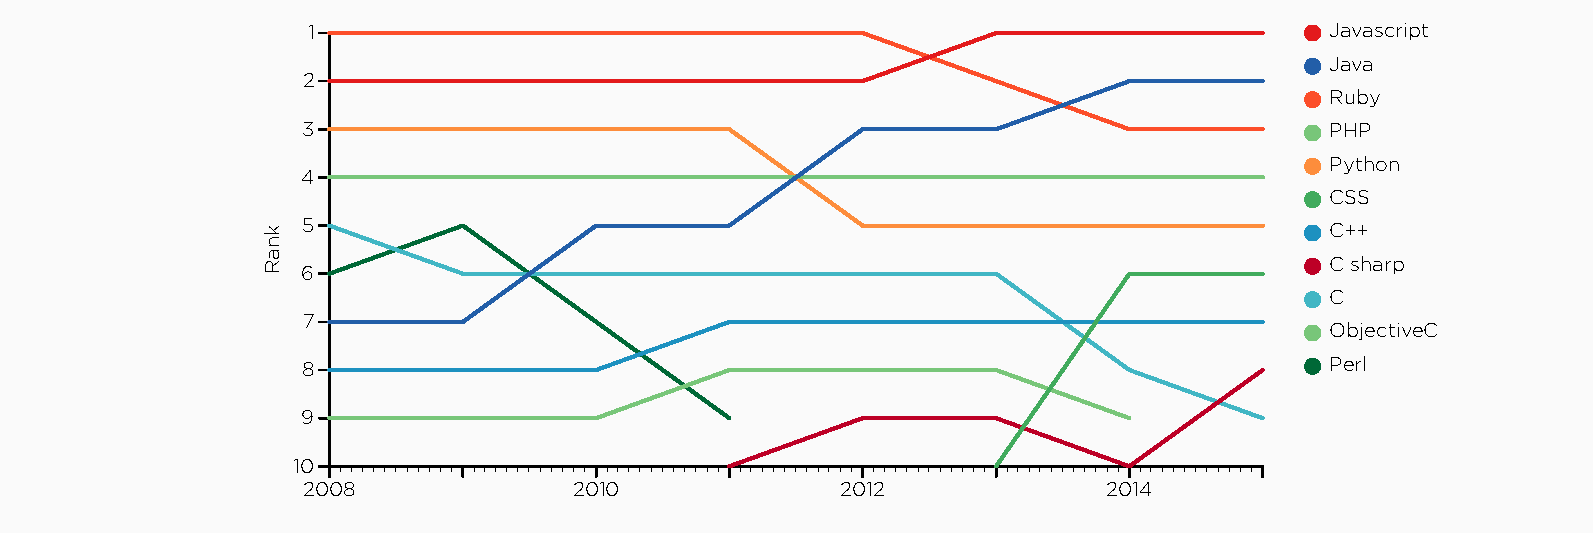
\includegraphics[width=\linewidth]{../resources/github-languages.pdf}
  \label{fig:github-languages}
  \caption{Languages Ranks from number of Github projects}
\end{figure}

% 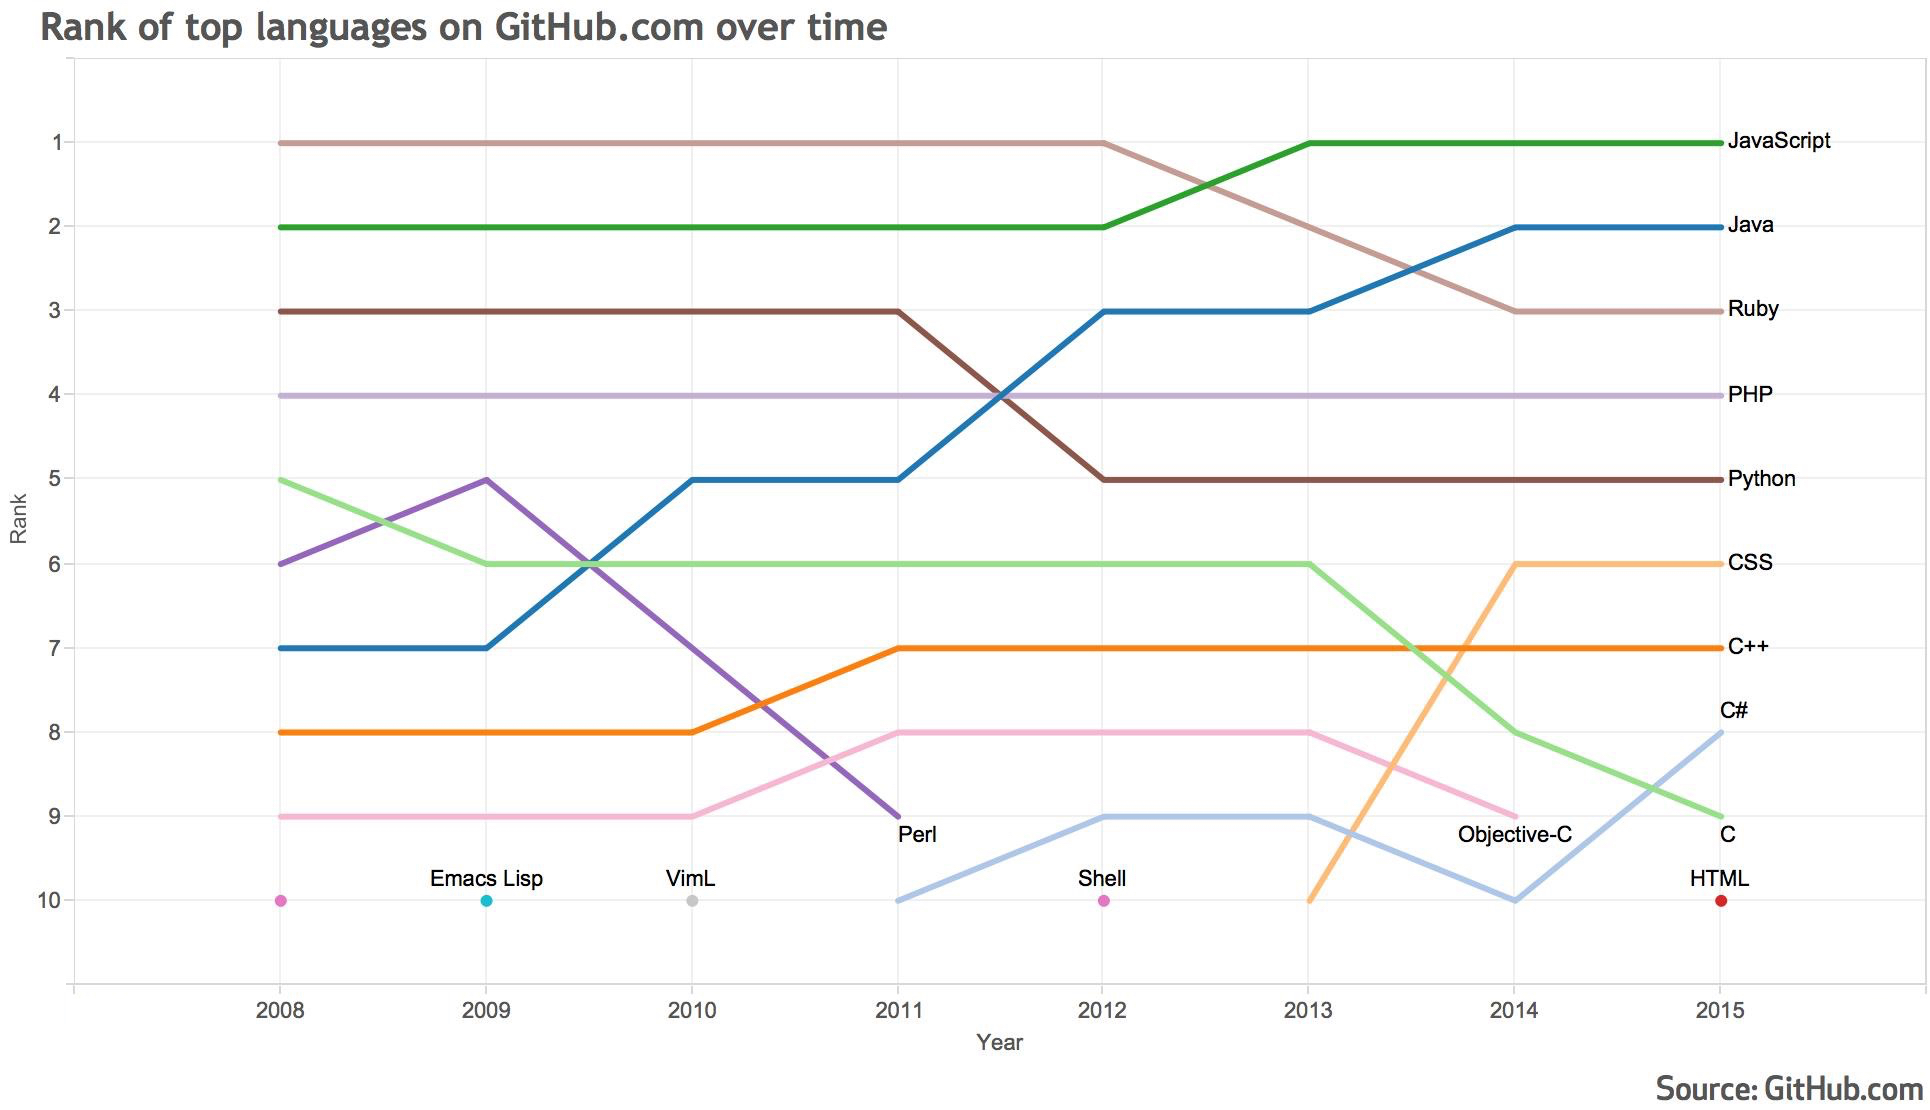
\includegraphics[width=0.9\linewidth]{../../data/js-trends/github-ranks}\ftnt{https://github.com/blog/2047-language-trends-on-github}

\nt{TODO graphical ranking of the tags in StackOverflow}

\begin{figure}
  \centering
  
\includegraphics[width=\linewidth]{../resources/stackoverflow-tags.pdf}
  \label{fig:so-tags}
  \caption{StackOverflow Tags evolution}
\end{figure}

% \nt{TODO redo this graph, it is ugly.}
% 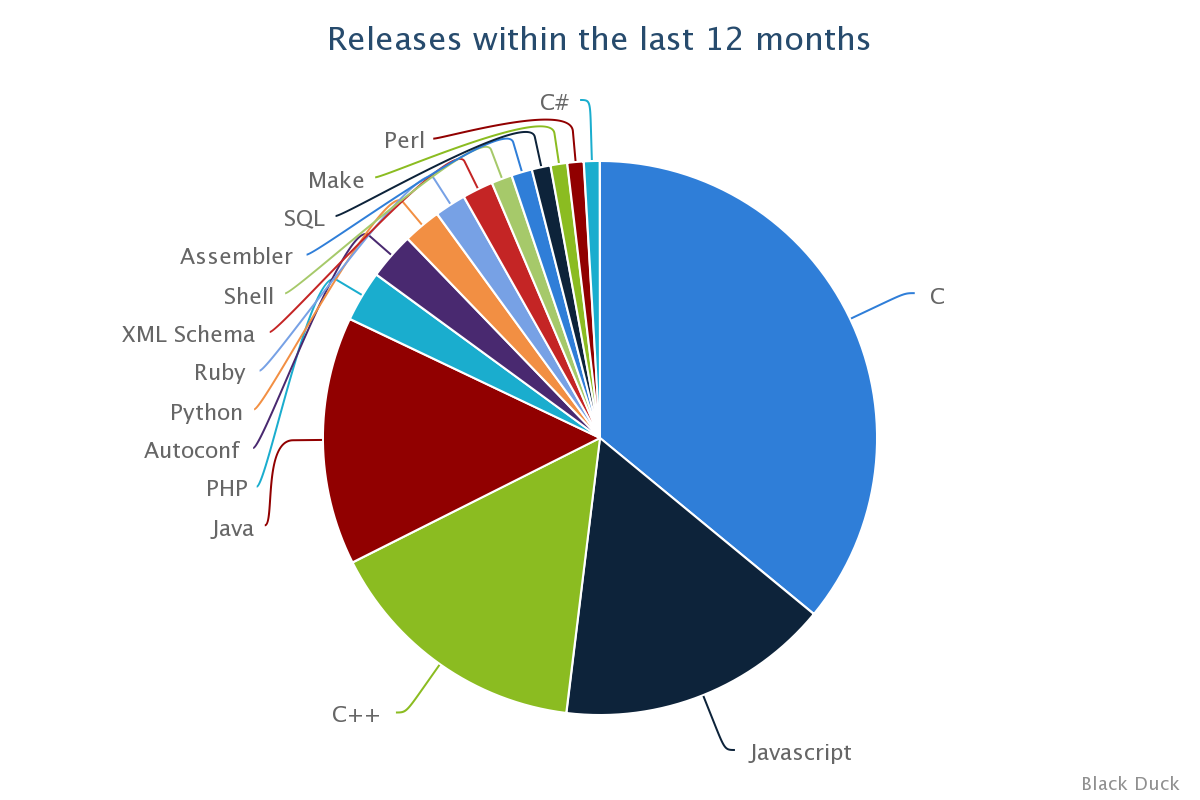
\includegraphics[width=0.9\linewidth]{../../data/js-trends/black-duck-15}

\begin{figure}
  \centering
  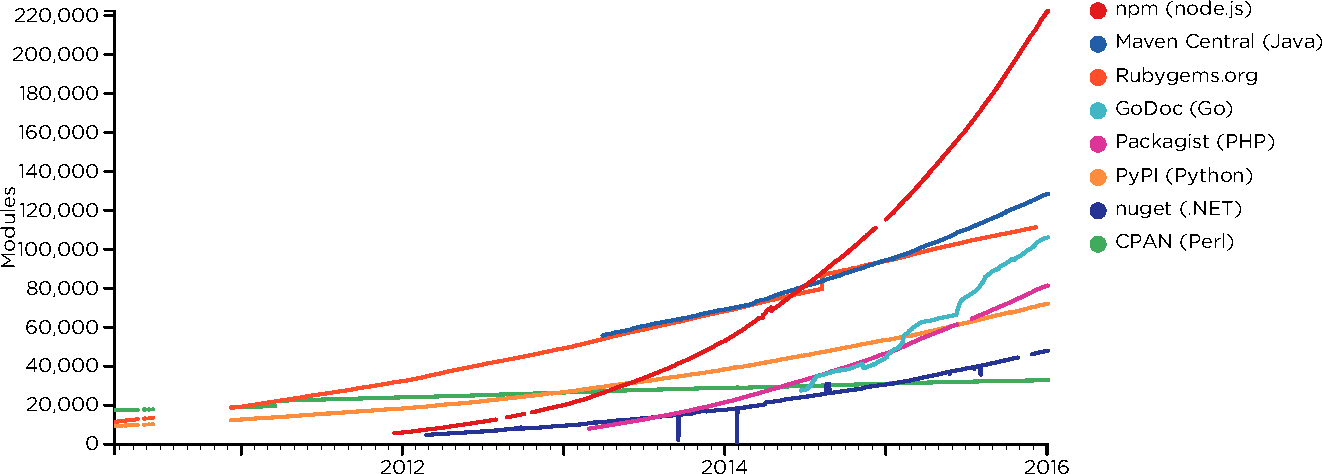
\includegraphics[width=\linewidth]{../resources/modulecounts.pdf}
  \label{fig:modulecounts}
  \caption{Module Counts per package manager}    
\end{figure}

\subsubsection{Industry}

The actors of the software industry tends to hide their activities trying to keep an edge on the competition.
The previous metrics represent the visible activity but are barely representative of the software industry.
The trends on job opportunities give some additional hints on the situation.
Javascript is the third most wanted skill, according to \textit{Indeed}\ftnt{http://www.indeed.com}, right after SQL and Java.\ftnt{http://www.indeed.com/jobtrends?q=Javascript\%2C+SQL\%2C+Java\%2C+C\%2B\%2B\%2C+C\%2FC\%2B\%2B\%2C+C\%23\%2C+Python\%2C+PHP\%2C+Ruby\&l=}
Moreover, according to \textit{breaz.io}\ftnt{https://breaz.io/}, Javascript developers get more opportunities than any other developers.
Javascript is increasingly adopted in the software industry.

\nt{TODO redo this graph, it is ugly.}
% 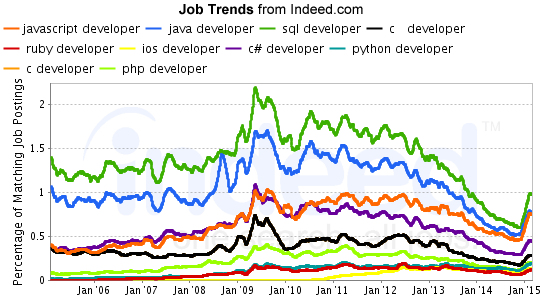
\includegraphics[width=0.9\linewidth]{../../data/js-trends/jobgraph}

\separator

Table \ref{tab:productivity-adoption} presents a summary of the analysis of the programming models presented in the previous paragraphs.

\ModularAdoptionTable{tab:productivity-adoption}

\subsection{Efficiency Limitations} \label{chapter3:software-productivity:efficiency-limitations}

Eventually, the presented languages are hitting a wall on their way to performance.

All the languages presented previously provide global memory abstraction on which to rely to assure encapsulation and composition -- either mutable state or immutable state.
Functional programming relies on immutable message-passing.
It might impacts performance at a fine-grain level because of heavy memory usage.
On the other hand, the synchronization required by mutable state is often hard to develop with \cite{Adya2002}, or avoid parallelism \cite{Pai1999,Krohn2007}.

The only solution to provide performance efficiency is to combine mutable state at a fine-grain level, with synchronization, and immutable state at a coarse-grain level, with message-passing.

% The next paragraph briefly presents the encountered incompatibility between modularity and performance to introduce the next section of this chapter.


% Parallelizing the execution increases the performances \cite{Amdahl1967,Gunther1993}
% But it is limited because accesses to sharing state need to be scheduled sequentially.
% Hence, to increase the parallelism and performance, the concurrent executions need to be independent, or to coordinate to be scheduled sequentially \cite{Gustafson1988,Gunther1996,Nelson1996,Gunther2002}.
% On the other hand, completely forbidding shared state, with immutable state, increase the need for communication because of the additional required synchronization.
% Eventually, the communications induce a greater overhead than the performance increases from parallelization, and it finally negatively impacts the performances.

% To be scalable, a solution needs to allow shared state at a fine grain, where lots of synchronization is required, and where communication would induce a greater overhead than parallelization could compensate. 
% And immutability at a coarse grain, where lesser synchronization is required, and parallelization can be advantageously used.

% Encapsulation aims not to provide this decomposition between sharing and immutable space required for performance scalability.
% It aims to draw a clear boundary around the concern of a module to help understanding it.
% To allow higher-order programming and mutable state, despite encapsulation, languages implement closures, and intermingle the memory between modules.
% It reinforces the need for synchronization and sequentiality.
% 
% Finally, the requirement to enforce the decomposition required for performance scalability are :
% \begin{itemize}
% \item shared state : fine level sequentiality
% \item immutable state : coarse level message passing
% \end{itemize}


The table \ref{tab:productivity-performance} presents the performance limitations of the languages presented in this section.
% It only presents programming languages.
The platforms extending these languages with concurrent or parallel features to provide performances are addressed in the next section.


\ModularEfficiencyTable{tab:productivity-performance}

\subsection{Summary} \label{chapter3:software-productivity:summary}

Table \ref{tab:productivity-synthesis} summarizes the characteristics of the solutions presented in this section.

\ModularSummaryTable{tab:productivity-synthesis}

\endinput






































\nt{read and include 
Octave and python: higher-level scripting languages productivity and performance evaluation, by Chaves, Nehrbass, Guilfoos, Gardiner.
Haskell vs Ada vs C++ vs Awk vs ... an experiment in software productivity, technical report by Hudak and Jones.
An empirical comparison of seven programming languages, by Prechelt.
}

% Pipeline parallelism is relevant for multi-pass algorithms \cite{Conway1963}, and it is particularly efficient for stream processing applications.

% \subsubsection{Efficiency Limitations} \label{chapter3:software-maintainability:limitations}


% Functional programming -> immutability is bad for performance at a fine grain because it implies lots of communication aka memory copy.
% Object Oriented Programming -> for the same reason, oop is not implemented in practice with message passing as the next section will present, even if the initial definition is about message passing.
% IMPORTANT -> immutability is bad for performance at a fine grain.


% Functional programming greatly support modularity to improve the maintainability of an application, and its resilience to evolution.
% However, the closures introduced by higher-order programming require to share the execution context among modules.
% The previous chapter show that sharing makes parallelism difficult.
% It is the reason why that maintainability and performance seem hardly compatible.
% This section explores in further details the limitation of modular programming regarding performances.

% \paragraph{Tighten Memory}

% Closures are implemented in languages using a global memory.
% And by exchanging closures, two modules intricately share their contexts of execution.
% Higher-order programming loosen the couple on the implementation level of the modules, but tighten it on the execution level.
% It improves modularity, but it inherently worsens the parallelization hence the performance scalability.

% \paragraph{Scalability Limitations}

% Parallelizing the execution increases the performances \cite{Amdahl1967,Gunther1993}
% But the parallelism is limited because the execution portions sharing state need to be scheduled sequentially.
% Hence, to increase the parallelism and performance, the concurrent executions need to be independent, or to coordinate to be scheduled sequentially \cite{Gustafson1988,Gunther1996,Nelson1996,Gunther2002}.
% We explain further the reasons of these limitations, and the improvement solutions in the next section.

% \nt{move this citation elsewhere}
% \cit{No matter how great the talent or efforts, some things just take time. You can't produce a baby in one month by getting nine women pregnant.}
% {Warren Buffett\ftnt{http://www.goodreads.com/quotes/476827-no-matter-how-great-the-talent-or-efforts-some-things}}


% \separator






\nt{TODO the transition is not very clear}
The modular organization of implementation is opposed to the organization favoring the parallelization of the execution.
The former organization supports the development scalability, while the latter supports performance scalability.
A program cannot trivially follow an organization that support both development evolution, and performance.
\nt{explain more clearly why}

The next section shows the improvements for performance and parallelism .
Then, section \ref{chapter3:software-performance} shows the techniques for parallelism.

\subsection{Efficiency Improvements} \label{chapter3:software-maintainability:performance}

INDUSTRY INDUSTRY INDUSTRY

To assure its integrity, the global state of an application imposes the concurrent executions to coordinate their accesses to be atomic and exclusive\nt{explain these terms}.
This coordination is responsible of the atomicity, and exclusivity of the accesses.
\nt{the next two sentences are not clear}
It assures the invariance of the state during its atomic manipulation.
So that developers can group operations in atomic manipulations so as to avoid corruption of the state.

The invariance is assured differently depending on how the state is shared among the concurrent execution.
To increase performance, concurrent executions needs to be as independent as possible to be executed in parallel \ftnt{http://joeduffyblog.com/2010/07/11/thoughts-on-immutability-and-concurrency/}.
% Isolation is independent processes
% Immutability Immutability
% Synchronization is event-loop, multi-thread, lock-free
\begin{description}
  \item[Isolation] If different concurrent executions are commutative \cite{Rinard1996,Clements2013a}, and they share no portion of the state then they can be isolated and executed in parallel.
  \item[immutable state] Otherwise, the sharing state portions needs to be immutable to conserve invariance and parallel execution \cite{Gordon2012,Matsakis2012a}.
  \item[shared state] If different concurrent executions needs mutation on the state, their accesses are scheduled sequentially.
\end{description}

\begin{center}
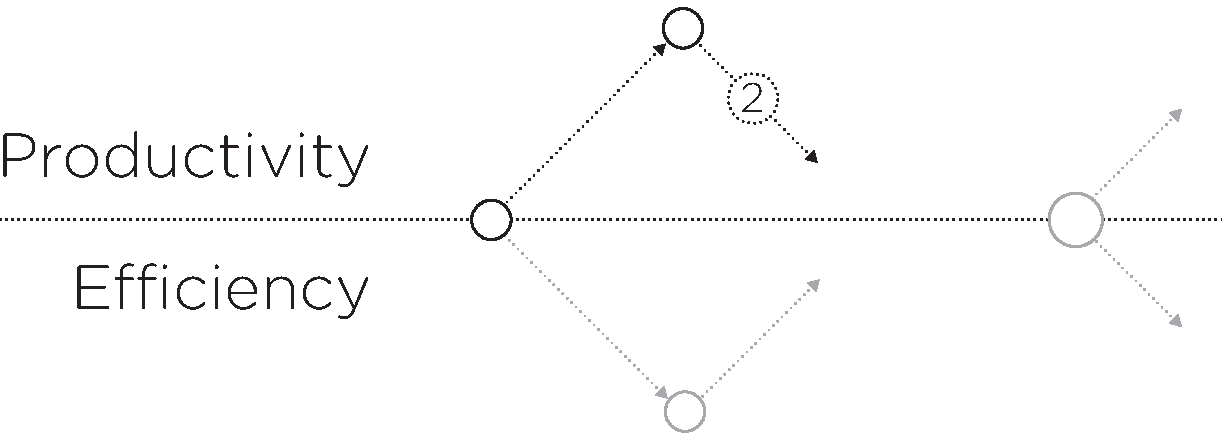
\includegraphics[width=0.6\textwidth]{../resources/state-of-the-art-2.pdf}
\end{center}

The next few paragraphs present the different models to assure invariance in concurrent execution, while conserving modular programming, \comment{as illustrated in the schema above}.
Section \ref{chapter3:software-maintainability:performance:concurrent-programming} presents the programming models providing synchronization and immutability for concurrent executions.
Section \ref{chapter3:software-maintainability:performance:compilation} presents compilation methods to parallelize sequential programs.

% Dynamic Isolation + Making asynchronous parallelism safe for the world \cite{Jr1990}


\subsubsection{Adaptation of the theoretical models to the industry}

The major program for modular programming is C, but it evolved with OOP into C++.
Nowadays, the major emblematic figures of OOP in the software industry are C++ and Java \cite{Gosling2000,Stroustrup1986}.
All these languages are far from the theoretical models proposed by the academy.
They get back to a more imperative model for performance reason.

Though, the trend seems to digress from these languages to evolve toward a more dynamic approach, closer to Functional Programming.
Functional programming like Haskell are not very efficient.
The major argument is that they are hell of a lot more expressive, but eventually, the lack of state is confusing and inefficient, and few developers adopt them.
Exactly like oop, or the actor model, immutability at a fine granularity is inefficient.
The good granularity is synchronization at a fine granularity (within functions), immutability and isolation at a coarse granularity (between modules).

Indeed Javascript adopts some functional features such as dynamic typing and higher-order functions \cite{Ecma1999}, because they are expressive, but conserve the state mutability for its performance.

The precedent chapter present the adoption of different languages, and particularly of Javascript.
No language from the academy is broadly adopted.
But more general / balanced / multi-paradigm languages are widely adopted (C/C++, Java, Javascript, Python etc ...).



% It is easy to understand the parallelism in a cooking recipe because the interdependencies between operations are trivial.
% It seems obvious that melting chocolate is independent from whipping up egg whites.
% % Because chocolate and egg whites are different ingredients.
% This distinction between chocolate and egg whites is trivial.
% % ... comes from the modifications to the state.
% While the distinctions within the state of an application are more intricate.
% This makes concurrent application more difficult to design and implement.


% \paragraph{Transition on parallel programming}

% The definition of separation of concerns given in this section is orthogonal to the original meaning coined by Dijkstra .
% It is interesting to note this difference, as it is related directly to this thesis.
% % Initially, it meant the ability to reason independently about different concern about a software system.
% The initial definition was about analyzing independently how a system meets different concerns.
% Dijkstra gives the example of analyzing independently correctness and efficiency.
% It is impossible to encapsulate correctness, or efficiency in a module, they concern the whole system.
% In this respect, this thesis is oriented towards dissociating the concern of development evolution and of performance.
% That is to be able to reason on the maintainability of a program, independently than of its performance, and vice versa.
% % This seems challenging as D. Parnas opposed these two concerns.
% It is the challenge presented by D. Parnas when he opposed the two concerns in \cite{Parnas1972}.

% This thesis investigates further this opposition to dissociate the concern of evolution and the concern of performance in the case of a web application.
% The next section investigates the first concern, and presents the major programming models used to improve the evolution of an application.

\endinput



remote first Zack Holman : promote asynchronous communication
\ftnt{http://zachholman.com/posts/remote-first/}
+
Conway's law
\cit{Organizations which design systems [...] are constrained to produce designs which are copies of the communication structures of these organizations.}
{M. Conway \cite{Conway1968}}



\subsubsection{Modularity based on Design Decisions}

Designing Software for ease of extension and contraction \cite{Parnas1979}

Design Rules: The Power of Modularity Volume 1 \cite{Baldwin1999}
A reference book, but I can't get it.

Promises 
\cite{Liskov1988}


What makes a great software engineer? \cite{Li2015}

About great software development:
Productivity : Sackman et. al 68, Gugerty & Olson 86
Collaboration, meaningful contribution : Kelly 99, Begel & Simon 06, Hewner & Guzdial 10
Communicate and acquire understanding : LaToza 06, Ko 06
Technical Knowledge : 
Open minded : McConnell 04, Bryant 13



Compiler productivity language into perfomance language
\cite{Kuper2015}\nt{TODO update biblio entry}
\section{Efficiency Focused Platforms} \label{chapter3:software-efficiency}

Both the academia and the industry proposed solutions with efficiency in mind to cope with the limitations the previous section concludes on.
Section \ref{chapter3:software-efficiency:concurrency} presents the concurrent and parallel programming paradigms, and their programming models. % oriented on performance rather than productivity.
Section \ref{chapter3:software-efficiency:adoption} presents the adoption steered by the efficiency of parallel programming.
Section \ref{chapter3:software-efficiency:productivity-limitations} presents the consequences of parallelism on productivity.
Finally, section \ref{chapter3:software-efficiency:summary} summarizes the three previous sections in a table.

\subsection{Concurrency} \label{chapter3:software-efficiency:concurrency}

\begin{figure}[!h]
\begin{center}
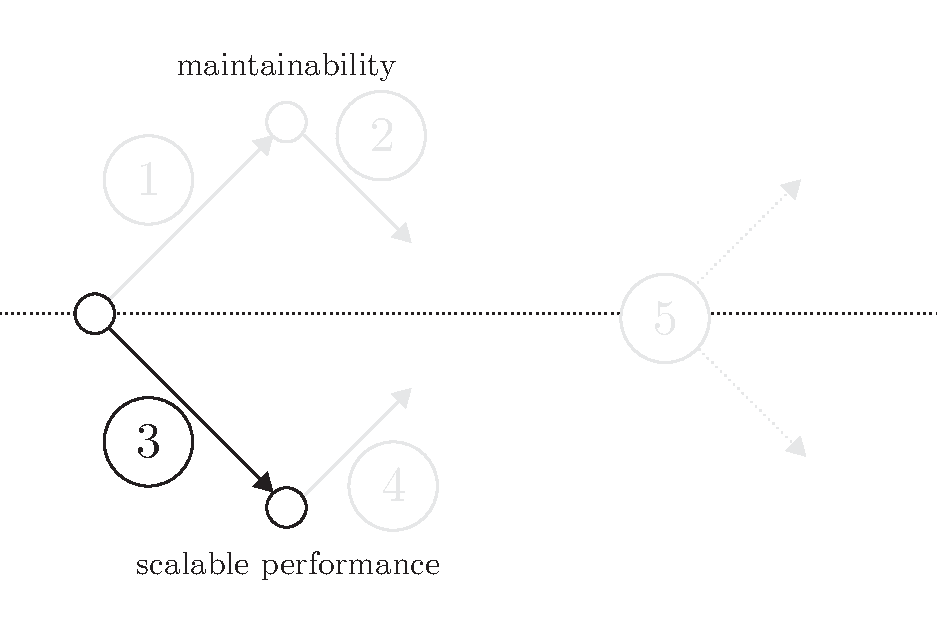
\includegraphics[width=0.6\textwidth]{../ressources/state-of-the-art-3.pdf}
\end{center}
\caption{Focus on Efficiency}
\label{fig:state-of-the-art-3}
\end{figure}

Web servers need to be able to process huge amount of concurrent operations in a scalable fashion.
Concurrency is the ability to make progress on several operations roughly simultaneously.
It implies to draw memory boundaries to define independent regions, or to define causality in the execution of tasks.
When both boundaries and causality are clearly defined, the tasks are independent and can be scheduled in parallel to make progress strictly simultaneously.

The definition of independent tasks allows the fine level synchronization within a task, and coarse level message passing between the tasks required for performance efficiency.
The synchronization of execution at a fine level assures the invariance on the shared state, and avoid communication overhead.
The message-passing at a coarser level assures the parallelism.
The two are indispensable for efficiency.

\subsubsection{Concurrent Programming} \label{chapter3:software-efficiency:concurrency:concurrent-programming}

% \cit{Building concurrent programming is like building a steam engine through a keyhole}{TODO}

\illustration{feu rouge et rond point}
Concurrent programming provides the mechanisms to assure atomicity of concurrent operations.
They define the causal scheduling of execution and assure the invariance of the global memory.
There are two scheduling strategies to execute concurrent tasks on a single processing unit, cooperative scheduling and preemptive scheduling.

\begin{description}
\item[Cooperative Scheduling] allows a concurrent execution to run until it yields back to the scheduler.
Each concurrent execution has an atomic, exclusive access on the memory.
\item[Preemptive Scheduling] allows a limited time of execution for each concurrent execution, before preempting it.
It assures fairness between the tasks, such as in a multi-tasking operating system.
But the unexpected preemption breaks atomicity, the developer needs to lock the shared state to assure atomicity and exclusivity.
\end{description}

The next paragraphs presents the programming model for these scheduling strategy, the event-driven programing model based on cooperative scheduling, and the multi-threading programming model based on preemptive scheduling.
Additionally, they present two alternatives to these two main programming models, lock-free data-structures and Fibers.

\paragraph{Event-Driven Programming}

Event-driven execution model queues concurrent tasks needing access to shared resources.
The tasks are explicitely defined by the developer.
The concurrent tasks are schedule sequentially to assure exclusivity, and cooperatively to assure atomicity.
% Web servers needs to be highly concurrent, and efficient.
It is very efficient for highly concurrent applications, as it avoids contention due to waiting for shared resources like disks, or network.
Several execution model rely on this execution model, like \ImplementationsOf{Event-driven programming}.
As well as some web servers like Flash \cite{Pai1999}, Ninja \cite{Gribble2001} thttpd\ftnt{http://acme.com/software/thttpd/} and Nginx\ftnt{https://www.nginx.com/}.

% However, a drawback of this model was that the execution context is lost at each event.
% The developer needs to explicitly transfer the relevant state to continue the execution from one event execution to another.

% + Fibers \cite{Adya2002}
% + Capricio \cite{Behren2003a} - User cooperative threads (also known as fibers / green threads)

% The problem of losing the execution context disappears with closures in higher-order programming.
% \nt{link with the previous paragraph}
% Moreover, the continuation passing style used in higher-order programming requires the developer to be aware of the asynchronous rupture in the execution, so as to assure atomicity \cite{Sussman1998}.
% And because an asynchronous call doesn't wait for the completion of the operation, the asynchronous control flow is not limited to be linear like in threads. \nt{more about that}
% Multiple asynchronous calls are made in parallel.

% + TAME \cite{Krohn2007} - event-based solution without stack ripping in C (it is like closure, but for C)
% + Node.js - \ftnt{https://nodejs.org/en/}
% + Vert.X - \ftnt{http://vertx.io/} node like + thread / worker capabilities

But the event-driven model is limited in performance.
The concurrent tasks share the same memory, and cannot be scheduled in parallel.
The next paragraph presents work intending to improve performance by reducing the atomic portions of operations to a minimum. % by reducing the sequential portions to a minimum to increase the possibilities of parallelism.

\paragraph{Lock-Free Data-Structures}

The wait-free and lock-free data-structures use atomic operations small enough so that locking is unnecessary \cite{Lamport1977,Herlihy1988,Herlihy1990,Herlihy1991,Anderson1990}.
They are based on instructions provided by transactional memories \cite{Harris2010} that combine read and write instructions,
They provide concurrent implementations of basic data-structures such as \ImplementationsOf{Lock-free Data-Structures}.

However these atomic operations are scheduled sequentially, which limits parallelism.
The next paragraphs present multi-threading, which, contrary to the event-driven model, requires the developer to explicitly define atomicity.
% using coarser granularity of atomic execution and exclusivity.

% Reference papers :
% Concurrent reading and writing \cite{Lamport1977}
% Impossibility and universality results for wait-free synchronization \cite{Herlihy1988}
% A methodology for implementing highly concurrent data structures \cite{Herlihy1990}
% Wait-free synchronization \cite{Herlihy1991}

% Book :
% The virtue of Patience: Concurrent Programming With And Without Waiting \cite{Anderson1990}

\paragraph{Multi-Threading Programming}

Threads are the small execution containers sharing the same memory execution context within an isolated tasks \cite{Dijkstra1968}, and scheduled in parallel with fork/join instructions \cite{Randall1998,Frigo1998,Leiserson2010}.
They execute statements sequentially waiting for completion, and are scheduled preemptively to avoid blocking the global progression.
The preemption breaks the atomicity of the execution, and the parallel execution breaks the exclusivity of memory accesses.
To restore atomicity and exclusivity, hence assure the invariance, multi-threading programming models provide synchronization mechanisms, such as \ImplementationsOf{Multi-threading programming}.

Developers tend to use the global memory extensively, and threads require to protect each and every shared memory cell.
This heavy need for synchronization leads to bad performances, and is difficult to develop with \cite{Adya2002}.

\paragraph{Cooperative Threads}

Cooperative threads, or fibers join the advantage of sequential waiting, with the advantage of cooperative scheduling \cite{Adya2002,Behren2003a}.
It avoids splitting the execution into atomic tasks nor use synchronization mechanisms to assure exclusivity.
A fiber yields the execution to another fiber to avoid blocking the execution during a long-waiting operation, and recovers it at the same point when the operation finishes.
However, developers need to be aware of these yielding operation to preserve the atomicity\ftnt{https://glyph.twistedmatrix.com/2014/02/unyielding.html}.

\paragraph{Limitation of Concurrent Programming}



% Moore's law \cite{Moore1965} which forecasts the density of transistors per processing unit, was wrongly interpreted to promise the exponential evolution in the sequential performance of the processing unit, and the assurance for the software industry of always faster hardware.
% But as transistors attained a critical size, the reduction in power required by transistor predicted by the Dennard's MOSFET scaling \cite{Dennard2007} stopped\ftnt{https://cartesianproduct.wordpress.com/2013/04/15/the-end-of-dennard-scaling/}.

Concurrent programming provides the synchronization required to assure sequentiality of execution within a task and the causal ordering between tasks.
However, multi-threading imposes sequentiality between tasks as well.
This global sequentiality is excessive ; it impacts performance, and is difficult to manage efficiently.

The causal ordering between tasks proposed by the event-driven execution model is sufficient to assure correctness of execution \cite{Lamport1978,Reed2012}.
But because of the lack of memory isolation, the concurrent tasks are not scheduled in parallel.

Parallel programming is the only solution for efficiency, at the expense of development efforts to explicitely define the memory isolation of concurrent tasks and their communications by message pasing.

% Synchronization mechanisms define shared memory, and lock-free data structures improve the parallel portion of execution, but the performance remains limited.

\paragraph{}

The table \ref{tab:efficiency-concurrency} presents a summary of the analysis of performance of the platforms presented in this section.

\ConcurrentEfficiencyTable{tab:efficiency-concurrency}



% Concurrent programming is a compromise to process operations simultaneously, by introduction synchronization to assure the exclusion required for shared states.


% The ever growing number of transistor predicted by Moore's law \cite{Moore1965} are arranged in parallel architecture to continue increasing the performance of processing units.
% Parallel programming became the only solution for efficiency, at the expense of development effort.


% This section presents the parallel programming solutions and their limitations in accessibility, and then the improvements to overcome these limitations.


% \nt{The shared-nothing architecture \cite{Stonebraker1986}}


\subsubsection{Parallel Programming} \label{chapter3:software-efficiency:concurrency:parallel-programming}


Concurrent programming allows to define the tasks scheduling causally.
% The ordering of operations is local within a synchronous execution, while the concurrent executions are causally ordered.
% It leads to parallel execution with some coordinations such as synchronization, immutability or isolation.
Concurrent tasks can be scheduled in parallel only if their memory are isolated.

The Flynn's taxonomy \cite{Flynn1972} categorizes parallel executions in function of the multiplicity of their flow of instruction and data.
Parallel programming models belong to the category Multiple Instruction Multiple Data (MIMD), which is further divided into Single Program Multiple Data (SPMD) \cite{Auguin1983,Darema1988,Darema2001} and Multiple Program Multiple Data (MPMD) \cite{Chang1997,Chan2004}.
SPMD defines a single program replicated on many processing units \cite{Culler,Johnson1995,K.ManiChandy2005} -- it is derived from the multi-threading programming model presented in section \ref{chapter3:software-productivity:concurrency:concurrent-programming}.
While MPMD defines multiple parallel tasks in the implementation \cite{Grimshaw1991,Foster1995b,Foster1996}.

\nt{schema of SPMD and MPMD}

% , communicating by message passing \cite{Sunderam1994,Snir1996,Walker1996}, SOAP, or the more recent REST protocols.

This section presents MPMD platforms allowing to define isolated tasks.
It presents theoretical and programming models on asynchronous communication and isolated execution for parallel programming.
It then presents stream processing programming models.
And finally, it concludes on the limitations of parallel programming regarding productivity. 



% % \paragraph{Asynchronous and Isolated Process Parallelism}

% The Flynn's taxonomy \cite{Flynn1972} is commonly used to categorize parallel executions.
% It separates the flow of instructions, and the flow of data, each being single or multiple.
% All the current parallel programming models belong to the category Multiple Instruction Multiple Data (MIMD), which is further divided into Single Program Multiple Data (SPMD) \cite{Auguin1983,Darema1988,Darema2001} and Multiple Program Multiple Data (MPMD) \cite{Chang1997,Chan2004}.
% % The difference between SPMD and MPMD holds on the distinction of instruction pool between the threads of execution.
% % SPMD implies to replicate the same program on all the processing units, while MPMD implies to define different programs for every processing units.

% \begin{figure}
% \begin{center}
% 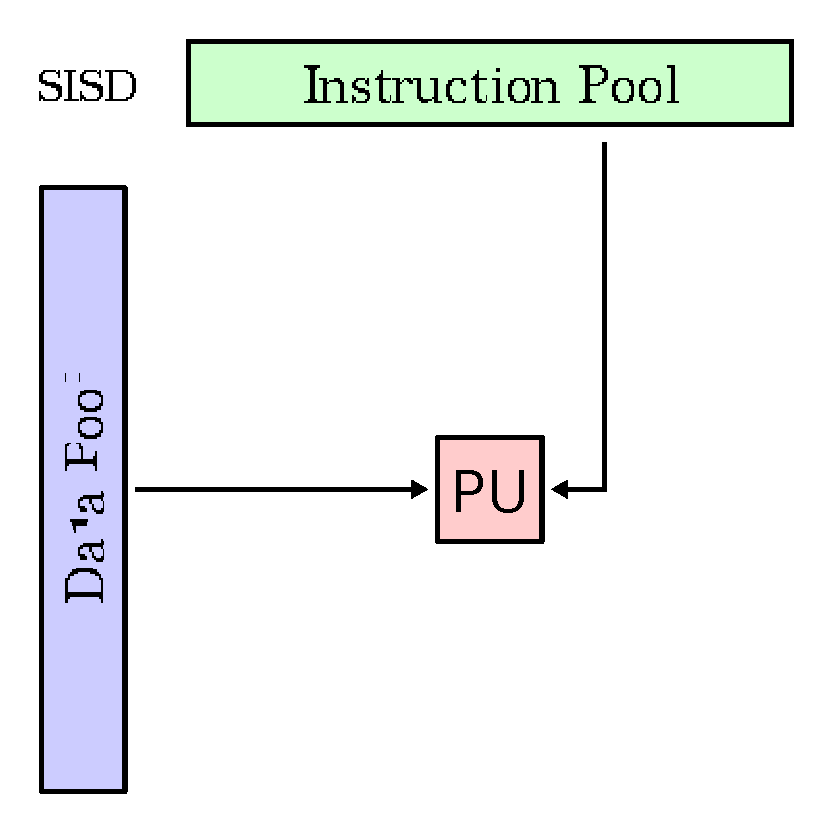
\includegraphics[width=0.2\textwidth]{../ressources/SISD.pdf}
% 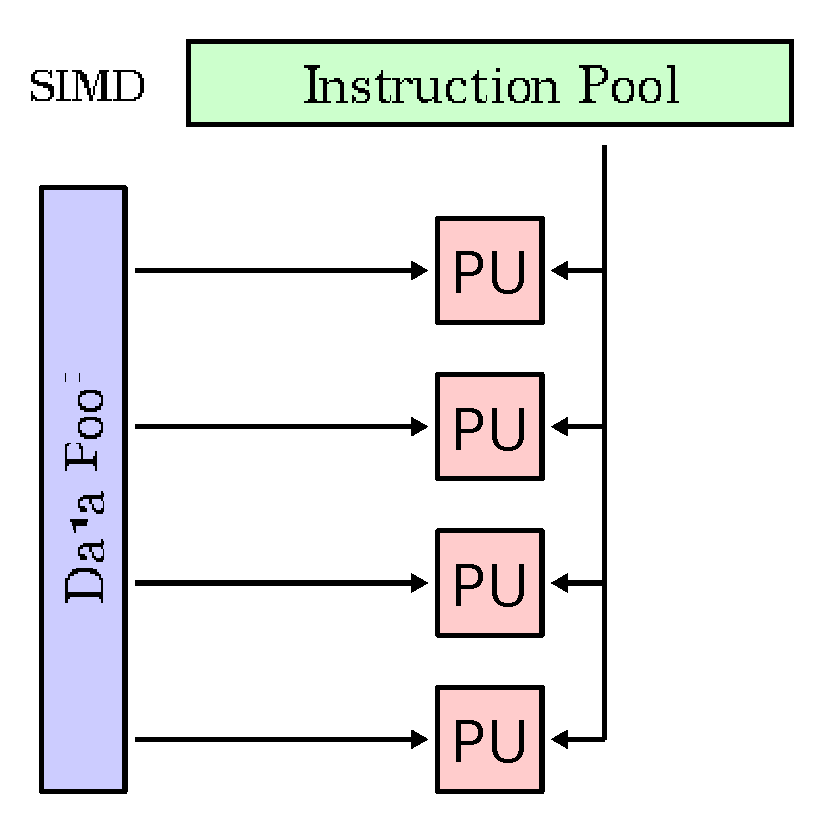
\includegraphics[width=0.2\textwidth]{../ressources/SIMD.pdf}
% 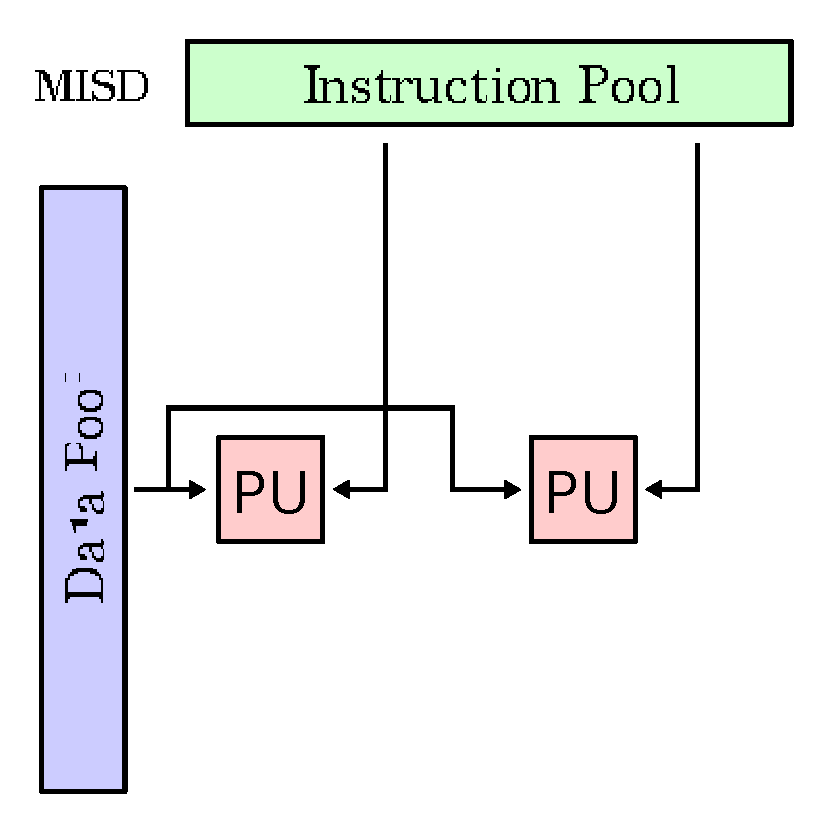
\includegraphics[width=0.2\textwidth]{../ressources/MISD.pdf}
% 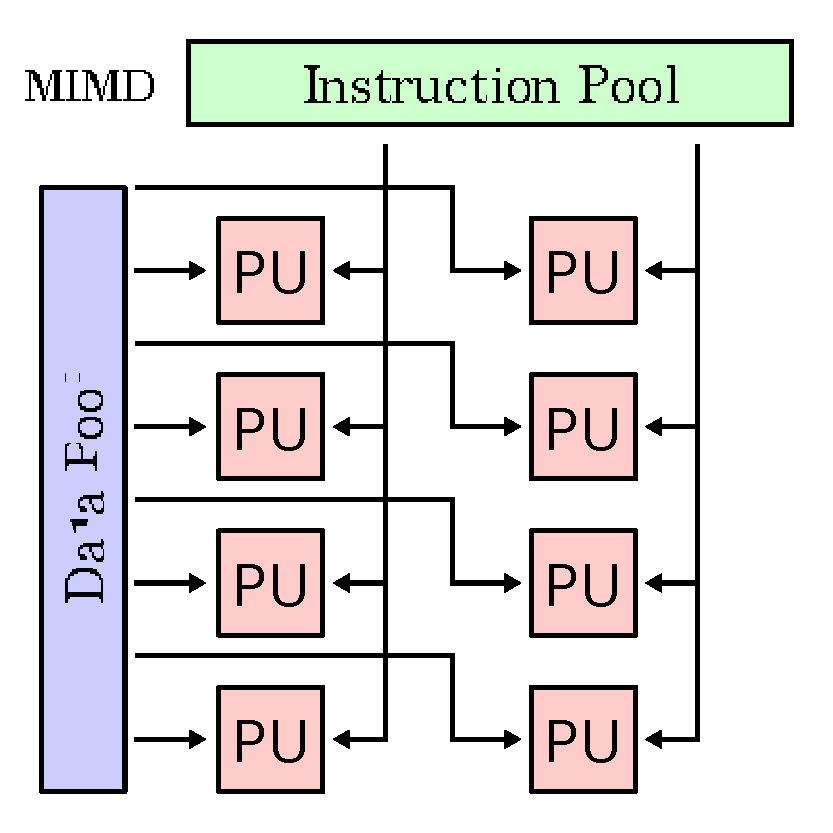
\includegraphics[width=0.2\textwidth]{../ressources/MIMD.pdf}\\
% by I, Cburnett. Licensed under CC BY-SA 3.0 via Commons
% \url{https://commons.wikimedia.org/wiki/File:{SISD,SIMD,MISD,MIMD}.svg}
% \end{center}
% \caption{Flynn's taxonomy of parallelism}
% \label{fig:flynn-taxonomy}
% \end{figure}


% % The difference between SPMD and MPMD is in the representation of the execution in implementation.
% SPMD defines a single program replicated on many processing units.
% Examples of SPMD programming languages are
% Split-C \cite{Culler},
% CRL \cite{Johnson1995} and
% Composite C++ \cite{K.ManiChandy2005}.
% %
% MPMD defines multiple processes in the implementation, communicating by message passing, using PVM \cite{Sunderam1994}, MPI \cite{Snir1996,Walker1996}, SOAP, or the more recent REST protocols.
% Examples of MPMD programming languages are
% Mentat \cite{Grimshaw1991},
% Fortran M \cite{Foster1995b} and
% Nexus \cite{Foster1996}.

% SPMD is close to the model presenting parallel improvements over modular programming presented in section \ref{chapter3:software-productivity:programming-models}.
% While MPMD is closer to the programming models based on isolated process presented in the remaining of this section.
% The coordinations between these processes is done by message passing, using PVM \cite{Sunderam1994}, MPI \cite{Snir1996,Walker1996}, SOAP, or the more recent REST protocols.

\paragraph{Theoretical Models}

The event-driven programming model used to cope with asynchronous communications allows the causal scheduling of concurrent tasks.
% The total ordering of execution imposed by sequential execution is excessive.
This causal scheduling is sufficient to assure correctness in a distributed system \cite{Lamport1978,Reed2012}.
% As Lamport showed \cite{Lamport1978}, and Reed related later \cite{Reed2012}, causal order is sufficient to execute correctly a system in parallel, such as a distributed system.
% The total ordering of execution provided by synchronization is an overkill.
The Actor model allows to express the causal ordering of computation as a set of parallel actors communicating by asynchronous messages \cite{Hewitt1973a, Hewitt1977, Clinger1981}.
In reaction to a received message, an actor can create other actors, send messages, and choose how to respond to the next message.
% All actors are executed concurrently, and communicate asynchronously.
% An asynchronous communication implies that the sender continues its execution immediately after sending the message, before receiving the result of the initiated communication.
Additionally, the communication in reality are too slow compared to execution to be synchronous, and are subject to various faults and attacks \cite{Lamport1982}.
The Actor model takes these physical limitations in account \cite{Hewitt1977a}.

% In the Actor Model, everything is an actor, even the simplest types like numbers.
% This level of granularity is unachievable in practice due to overhead from the asynchronous communications.
% Most implementations adopt a granularity on the process or function level.

Similarly, coroutines are autonomous programs which communicate with adjacent modules as if they were input and output subroutines \cite{Conway1963}.
It defines a pipeline to implement multi-pass algorithms.
Similar works include the Communicating Sequential Processes (CSP) \cite{Hoare1978, Brookes1984}, and the Kahn Networks \cite{Kahn1974, Kahn1976}.

\subsubsection{Summary of Concurrent and Parallel Programming Models}

Table \ref{tab:efficiency-parallel} presents a summary of the analysis of the paradigm presented in the previous paragraphs.

\ParallelEfficiencyTable{tab:efficiency-parallel}







\subsection{Adoption} \label{chapter3:software-efficiency:adoption}

\begin{figure}[!h]
\begin{center}
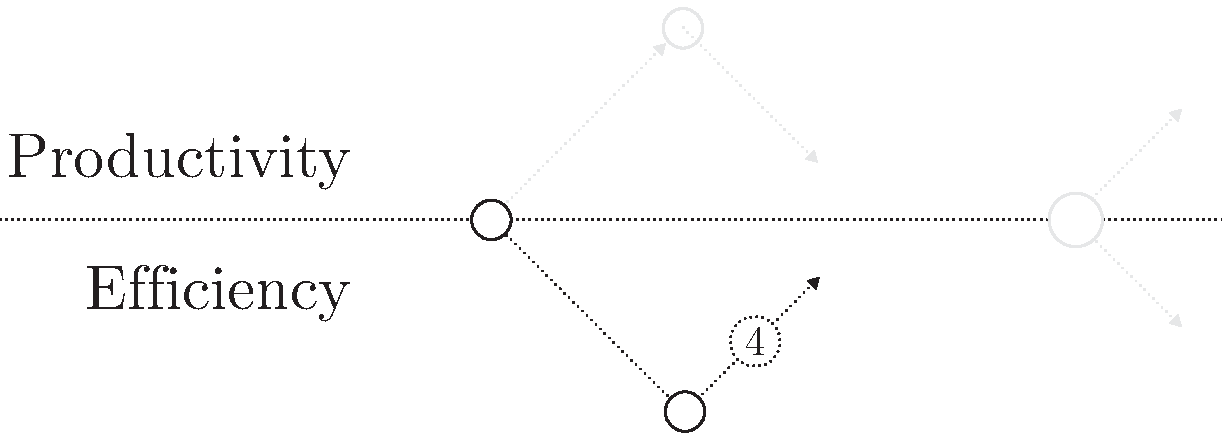
\includegraphics[width=0.6\textwidth]{../ressources/state-of-the-art-4.pdf}
\end{center}
\caption{Steering back toward Productivity}
\label{fig:state-of-the-art-4}
\end{figure}


\illustration{mars rover}
When the need for efficiency is higher than the need for productivity, the adoption is steered by the industry more than the community.
If the industry really needs a platform, it will commit the required development effort despite a low productivity.
% If there is industrial need, there will be maintenance.
The platforms for the Mars Rover or the banking systems are 30 years old, yet the industry continues to maintain them.
%, and there is no community to maintain it.
The platform presented in this section emerged from the academia and the industry but are often barely known by the larger community of developers.
The more the platform abandons productivity, the less it will be supported by the community.

% The performance improvements comes directly from the industry requirements.

% All these system make sense in industrial context.
% Industries have the money to fund the necessary research.

% However, the context of this thesis is different from a classical industrial context.
% During the bootstrap of a web application project, the economical context requires technologies with strong community, to pick talents from to grow the team quickly and effortlessly.
% It also requires these technologies to be of industrial standard, to build a reliable product.
% And these technology must be compatible with web technologies.
% \begin{itemize}
% \item Community support
% \item Industrial need
% \end{itemize}


% \nt{review this paragraph and the transition to the next section}
% The field of concurrent programming is so vast it is impossible to relate here every programming languages.
% The previous examples are only the best known.
% The next focus focuses on streaming real-time applications.

% \comment{transition on lazy evaluation equivalence to stream. lazy evaluation + side effects + concurrency = streams}



% + all the solutions that have a great industrial impact (storm, millwheel and co)



% \subsubsection{Exection Decomposition}


% The programming paradigms presented above are implemented in many existing programming languages.
% All major programming languages implements some form of concurrency or parallelism mechanism.
% The next paragraphs presents these implementations by the industry and the community.
% And more specifically, how they deal with the need to decompose the execution.

% \paragraph{Event-Loop}

% The event-loop model, featured by the DOM and Node.js with Javascript, allows concurrency but not parallelism.
% It decomposes the execution into sequences of callbacks functions, but keep the memory shared.

% As presented in the previous section, Javascript is currently one of the most used language.
% This asynchronous programming model without the memory decomposition seems to be easy to develop with.
% It is used extensively in the community as well as in the industry.
% However, when the programming model requires the memory to be decompose, in order to get parallelism, it becomes more complicated to develop with, as presented in the next paragraphs.

% \paragraph{Multi-Threading}

% The multi-threading model allows concurrency and parallelism on certain execution region.
% It decomposes the execution into fork-join threads, and the memory is shared, but protected with locks.
% The protection of the shared memory is the reason concurrent programming is difficult to manage for most developers.
% Multi-threading is difficult to program with, and for this reason, it leads to poor performances.
% It is not heavily used in the community, where the need for concurrency is limited.
% In the industry, where the concurrency is often required, multi-threading is abandoned for other paradigms, such as the event loop or the actor model.

% \paragraph{}

% The event-loop requires an execution decomposition, but not a memory decomposition.
% This paradigm is heavily adopted by both the community and the industry.
% On the other hand, the multi-threading paradigms with locks requires an execution decomposition, and light memory decomposition.
% This paradigms is not heavily used in the community, and is being abandoned by the industry.
% This comparison between the event-loop and the multi-threading paradigms seems to indicate that the memory decomposition heavily restrains the adoption by the community.
% Hence, it impacts the productivity required for the adoption in the economical context of this thesis, as shown in table \ref{scalability-execution-decomposition}.

\subsubsection{Concurrent Programming}

Most programming languages implementation supports concurrent programming somehow.
Either with multi-threading or event-driven programming.
These two are highly adopted by both the industry and the community, as presented in section \ref{chapter3:software-productivity:adoption}.

On the other hand, lock-free data structures and cooperative threads comes from the academia, similarly to functionnal programming, and did not encounter significant adoption from the community.

Table \ref{tab:adoption-concurrent} presents a summary of the adoption of concurrent programming models.

\ConcurrentAdoptionTable{tab:adoption-concurrent}

\subsubsection{Parallel Programming}

There exists several platforms directly inspired by the actors model, like \ImplementationsOf{Actor Model}.
Scala is a programming language unifying the object model and functional programming.
Akka is a framework based on Scala, following the actor model to build highly scalable and resilient applications.
Play is a web framework based on top of Akka.
And Erlang is a functional language designed by Ericsson to operate networks of telecommunication devices \cite{Armstrong1993,Nelson2004,Armstrong2014}
% Nelson2004 is not very good, find another better citation.

There are as well other platforms inspired by other theoretical model, like \ImplementationsOf{Concurrent Sequential Processes}, inspired by Coroutines and CSP.
Go is an open source language initiated by Google to build highly concurrent services.

These examples of implementation are largely used in the industry, but are almost unknown outside of it.
They are backed by strong, but small passionated communities.

However, the organization in independent tasks is hardly compatible with the modular organization presented in the previous section.
It is difficult for developers to manage the superposition of these two organizations, tasks and modules.
This superposition makes these platforms accessible only to an elite in the industry supporting it.
The next paragraphs present platforms mitigating the difficulty stemming from the duality between execution decomposition and modularity.

\paragraph{Tasks Organization and Communications}

To reduce the difficulties of the superposition of tasks and modules, algorithmic skeletons propose predefined patterns of organization to fit certain types of problems \cite{Cole1988, Dean2008, McCool2010, Gonzalez-Velez2010}.
Developers specialize a skeleton and focus on their problem independently of the required communication.
These solutions are hardly used by the community, but are crucial in some industrial contexts.
A famous example is the map/reduce pattern introduced by Google \cite{Dean2008}.

% \nt{Link with DSMS}
% As there is similtudes between SQL-like languages, functional structures, and algorithmic skeletons, the latter can be seen as a tentative to merge the more descriptional features of the former into imperative programming.
% Indeed, among the Algorithmic skeletons, we can cite Map / reduce, which are functional structures, but are somehow equivalent to the select and aggregate functions of SQL.
% The pipeline architecture for data stream processing presented in section \ref{chapter3:software-efficiency:dataflow-pipeline} can be considered as algorithmic skeletons.

% However, they introduce limitations and difficulties, as the developer must fit its problem into the skeletons.
% One of this difficulties, it that a common memory is impossible to use.
% Developers needs to think in terms of message passing instead of a global memory, which, as we saw in previous section, is incompatible with best practices.

% Introducing 'Bones': a parallelizing source-to-source compiler based on algorithmic skeletons \cite{Nugteren2012}

\paragraph{Tasks Granularity}

The Service Oriented Architectures (SOA) allows developers to express an application as an assembly of services connected to each others.
Some examples of SOA platforms are \ImplementationsOf{Service Oriented Architecture}.
It allows to adjust the granularity of tasks to help developers to better fit the tasks organization with the modular organization \cite{Adam2008}.

More recently, Microservices are tackling the same challenge on the web \cite{Fernandez-Villamor2010,Fowler2014,Namiot2014}.
Some examples of Microservices are \ImplementationsOf{Microservices}.
They are very recent, and it is difficult to asses their usage in the community nor the industry.
But they seems to be increasingly adopted, both in the industry and in the community.

% In modular programming a module protects the rest of the implementation from the consequences of the design choice its encapsulate, while a service encapsulate a specific task, with possible consequences on the adjacent services.

% In a fine enough granularity of service, each service becomes so simple, it can limits the consequences of its modification.

\paragraph{}

The parallel programming platforms previously presented allow to build generic distributed systems.
In the context of the web, a real-time application must process high volumes streams of requests within a certain time.
The next paragraphs present platforms focusing on this challenge.
% Because these systems are key to business, their reliability and latency are of critical importance.
% The next paragraphs present the platform meeting these requirements required for industry adoption.
% Again, these platforms emerged from the academia and the industry and did not always gather huge community enthusiasm.


\subsubsection{Stream Processing Systems}

% Otherwise, input data may be lost or output data may lose their value.
% These requirements are challenging to meet in the design of such system.

\paragraph{Data-stream Management Systems}

Database Management Systems (DBMS) historically processed large volume of data, and they naturally evolved into Data-stream Management System (DSMS) to processed data streams as well.
Because of this evolution, they are in rupture with MPMD platforms presented until now.
They borrows the syntax from SQL to run requests in parallel on continuous data streams.
The computation of these requests spread over a distributed architecture.
% Among the early works, we can cite
% NiagaraCQ \cite{Chen2000,Naughton2001},
% Aurora \cite{Abadi2003,Abadi2003a,Balakrishnan2004} which evolved into
% Borealis \cite{Abadi2005},
% AQuery \cite{Lerner2003},
% STREAM \cite{Arasu2003,Arasu2005} and
% TelegraphCQ \cite{Krishnamurthy2003,Chandrasekaran2003}.
% More recently, we can cite
Some recent examples are \ImplementationsOf{Data Stream System Management}.


\paragraph{Pipeline Architecture}

% As presented in the previous section, streaming composition allows a loosely coupled yet efficient composition.
The pipeline architecture introduced by SEDA \cite{Welsh2001} organizes an application as a network of event-driven stages connected by explicit queues, the output of one feeding the input of the next.
The event-driven paradigm of a stage is similar to work like Ninja \cite{Gribble2001} and Flash \cite{Pai1999} previously presented.
But the independence of stages allow to spread the execution on a parallel architecture.
% SEDA is the precursor in the design of pipeline-based architecture for real-time web applications.
The academic works and industrial implementations of pipeline architecture are \ImplementationsOf{Pipeline Architecture}.

% Storm \cite{Toshniwal2014} is designed by and used at Twitter to process the heavy streams of tweets.
% It is only one example of industrial practical application, among many others.

\paragraph{}

Parallel programming is barely supported by the community, but emerges mainly from industrial needs and academic research.
The implementations improve efficiency, but prevent their adoption by the community due to a weak productivity.
Despite the performance limitation, the event-driven programming model is the best candidate for a concurrent programming model supported by the community, and with concrete needs in the industry.
Table \ref{tab:efficiency-adoption} summarize the adoption of the platform oriented toward performance presented in this section.

\ParallelAdoptionTable{tab:efficiency-adoption}

\subsection{Productivity Limitations} \label{chapter3:software-efficiency:productivity-limitations}

Parallel programming requires the organization of execution and memory into independent tasks.
It allows the different granularity of state accessibility required for efficiency.
At a fine level, the state is shared, while at a coarser level, it is isolated.
This difference in state access impacts higher-order programming.
It limits the composition of modules, hence impacts productivity.
% id dictated by the execution organization in tasks.
% prevent higher-order programming between tasks, hence impacts productivity.

% Indeed, the topology of the network of actors is statically defined, and the dynamical modification of the topology is mostly impossible.
% It is not possible to dynamically manipulate execution containers, like it is possible to manipulate functions.
% Therefore, higher-level programming is impossible, and limits the modularity required for productivity.
Without good composition between modules, parallel programming forces to develop two mental representations -- one for the module organization and one for the tasks organization -- or to abandon the module organization and productivity altogether.
% The memory decomposition required by parallel programming is hard to manage, and 
It makes parallel programming productive only to an elite of developers that are able to keep the two mental representations.

This thesis focus on platforms allowing developers to be productive, and to produce efficient web applications to stimulate the economy.
To fit the economical context of this thesis, a solution must provide efficiency while avoiding the developers to keep a double mental representation of the implementation.
It comes with an abstraction for the tasks and memory organization, for the developer to focus only on the module organization providing productivity.
The next section presents some works that provides such an abstraction.

\EfficiencyProductivityTable{tab:efficiency-productivity}


\subsection{Summary} \label{chapter3:software-efficiency:summary}

Table \ref{tab:efficiency-synthesis} summarizes the characteristics of the platforms presented in this section.

\EfficiencySummaryTable{tab:efficiency-synthesis}

\endinput







TO READ :

Streaming
\cite{Madsen2015}
\cite{Sun2015}

Map Reduce
\cite{Yao2015}


Web assembly
https://medium.com/javascript-scene/what-is-webassembly-the-dawn-of-a-new-era-61256ec5a8f6












\endinput

\subsection{Concurrency Theory} \label{chapter3:parallel-execution:concurrency-theory}

The mathematical models are a ground for all following work on concurrent programming, we briefly explain them in the next paragraphs.
There are two main formal models for concurrent computations.
The Actor Model of C. Hewitt and the Pi-calculus of R. Milner.
Based on these definitions, we explain the importance of determinism for correctness, and the reasons that made asynchronous message-passing prevail.

% TODO illustration of cells, and draw an analogy between cells and actor model.
% Or something the actor models is based upon.

\subsubsection{Models}

\paragraph{Actor Model}

The Actor model allows to express the computation as a set of communicating actors \cite{Hewitt1973a, Hewitt1977, Clinger1981}.
In reaction to a received message, an actor can create other actors, send messages, and choose how to respond to the next message.
All actors are executed concurrently, and communicate asynchronously.
% The Actor model uses an asynchronous message-passing communication paradigm.
% The communication between two actors, the sender and the receiver, is a stream of discrete messages.
% The sender names the receiver actor when sending messages to be the recipient of these messages.
An asynchronous communication implies that the sender continues its execution immediately after sending the message, before receiving the result of the initiated communication.

The Actor model was presented as a highly parallel programming model, but intended for Artificial Intelligence purposes.
Its success spread way out of this scope, and it became a general reference and influence.
% For example, the Scala programming language features an actor approach to concurrency.

% More recent work of C. Hewitt on Actors is about ... \nt{TODO} \cite{Hewitt2007,Hewitt2007a}.

\paragraph{$\pi$-calculus}

R. Milner presented a process calculus to describe concurrent computation : the Calculus of Communicating Systems (CCS) \cite{Milner1975, Milner1980}.
It is an algebraic notation to express identified processes communicating through synchronous labeled channels.
% In CCS, process compose concurrently, communications are synchronous, and the topology is static.
The $\pi$-calculus improved upon this earlier work to allow processes to be communicated as values, hence to become mobile \cite{Engberg1986,Milner1992a,Milner1992}.
Therefore, similarly to Actors, in Pi-calculus processes can dynamically modify the topology.
However, contrary to the Actor model, communications in Pi-calculus are based on simultaneous execution of complementary actions, they are synchronous.


% Actors can create actors, pi-caclulys processes can replicate, and send processes through channel.
% Processes create a new processes on each instruction to continue the execution.!g systolic arrays

% Pi-calculus resembles to the actor model, but its algebraic nature led to a critical difference with the latter.
% Indeed, processes in the Pi-calculus communicate indirectly, through labeled ports, whereas actors communicate directly by naming the recipient actors.
% This difference allows multiple processes to listen in turns to the same channel, whereas the recipient of a message cannot change.

% I think this difference lead the Pi-calculus to be composable, whereas message-passing is not.
% Message-passing is not composable, whereas invocation is.
% The Actor model is not an ideal programming model, as non-composability makes difficult to reuse or extends existing components.
% A way to compose actors, is to send to an actor the name of the actor to respond to.
% It is similar in essence to the continuation concept.








\section{Reconciliations} \label{chapter3:reconciliations}
\nt{TODO title not clear enough}

\subsection{Contradiction}

The decomposition of an application into a pipeline, as shown in the two previous sections, is incompatible with the modular design advocated by the separation of concerns.
The problem of incompatibility between the modular design and the parallel execution of a pipeline architecture is the following.
There need to be a common understanding on the structure of the communication from one stage to the next.
The modular design defines that this common ground, the interface, be the most resilient possible to focus the evolution within a module.
While the pipeline architecture (and more generally the concurrent programming models) defines these interfaces as the communications between the stages of the execution.
With the evolution of the problem specification, when a stage needs to be modified, it is most likely that these changes will affect the previous or next stages.
% which will eventually change with the evolution of the problem specification.

Most project use languages supporting the modular design at the beginning, when they need to evolve the most.
They then switch to the pipeline architecture only when the requirement of performance overcomes the requirement of evolution.
Moreover, as the team knows that they will eventually throw away their code to upgrade it to a different paradigm, there is little effort to follow the best practice to make maintainable code.
It results in a large effort of development to compensate this rupture.
% This rupture between the two organization is not novel, and is at the center of a large body of work.
In this section, we present the state of the art to reconciliate the two organizations, and avoid this rupture.
First we see the design patterns to fit both organization onto a same source code.
Then we see the compilation tentatives to switch from one to the other.
\section{Adoption Focused Platforms} \label{chapter3:software-adoption}

Section \ref{chapter3:software-productivity} and section \ref{chapter3:software-efficiency} present the platforms focusing respectively on productivity and efficiency, and conclude that favoring on one negatively impacts the other.
Moreover, a balance between productivity and efficiency is required to be both supported by the community and needed by the industry, hence trigger a virtuous circle of adoption.
This section presents platforms featuring an abstraction of the tasks organization to allow developers to focus on the modular organization to keep both productivity and efficiency.
Section \ref{chapter3:software-adoption:compilers} presents Compilers, and section \ref{chapter3:software-adoption:runtimes} presents Runtimes.

% \nt{read and include \cite{Catanzaro2009} it is about Productivity language JIT compilation into efficient language
% And get all the paper that cite this one.}
% \nt{read and include \cite{Engler1994}}
% \nt{read and include \cite{Kovachev2011}}
% \nt{read and include \cite{Asanovic2006}}

\begin{figure}[!h]
\begin{center}
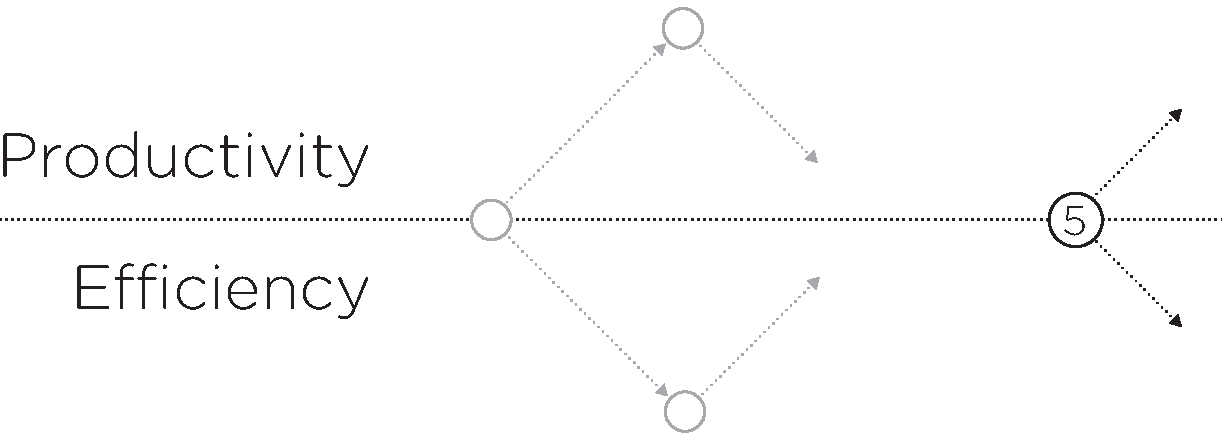
\includegraphics[width=0.6\textwidth]{../resources/state-of-the-art-5.pdf}
\end{center}
\caption{Focus on Adoption}
\label{fig:state-of-the-art-5}
\end{figure}

\subsection{Abstraction of Tasks Organization}

\subsubsection{Compilers} \label{chapter3:software-adoption:compilers}

\cit{It is a mistake to attempt high concurrency without help from the compiler}{R. Behren, J. Condit, E. Brewer \cite{Behren2003}}.

As soon as the incompatibility between the modules and the tasks organizations were presented, it was suggested to use a compilation approach to mitigate this incompatibility \cite{Parnas1972}.
% When showing the incompatibility between the two organization, D. Parnas  advocated conciliating the two methods using an assembler to transform the development organization into the execution organization \cite{Parnas1972}.
This section presents the state of the art to extract parallelization from sequential programs through code transformation and compilation.

\nt{read and include \cite{Catanzaro2009}}

\paragraph{Parallelism Extraction}

Extracting parallelism from a sequential implementation is a hard problem \cite{Johnston2004a}.
A compiler needs to identify the commutative operations to parallelize their executions \cite{Rinard1996,Clements2013a}.

An important work was done to parallelize loop iterations \cite{Mauras1989,Amarasinghe1995,Chen2008,Banerjee2013,Radoi2014}, particularly using the polyhedral compilation method \cite{Bastoul2004}.
Examples of polyhedral compilers are \ImplementationsOf{Polyhedral Compilers}.
To improve performance gains outside of loops, some compilers identify the data-flow parallelism on the whole program \cite{Beck1991,Catanzaro2009,Li2012}.
Moreover, the data-flow representation and execution of a program is well suited for modern data processing applications \cite{Fernandez2014a}, as well as web services \cite{Salmito2013}.
% \nt{TODO Extract parallelism compilers from these :
% Load balanced pipeline parallelism \cite{Kamruzzaman2013}, 
% Regent \cite{Slaughter2015},
% Cilk-P, On-the-Fly Pipeline Parallelism\cite{Lee2013}
% }

% However, the limitation of modular programming regarding parallelization persists.
% In a purely functional language with immutability, higher-order functions are referentially transparent which implies commutativity hence parallelism \nt{Add reference of parallel purely functional languages}.
% \cite{Herrmann2000}
Mutable closures required for higher-order programming remains a challenge to parallelize because of the memory references shared across the program \cite{Harrison1989, Nicolay2010, Matsakis2012a}.
The next paragraphs present some improvements in compilation applicable for parallelism extraction.
% The first paragraph presents static analysis, while the second presents annotations systems.

% - Continuation-passing style parallelization compilation \cite{Harrison1989}.The interprocedural analysis and automatic parallelization of Scheme programs
% - Automatic Parallelization of Scheme Programs using Static Analysis \cite{Nicolay2010}

% - Commutativity analysis: A new analysis framework for parallelizing compilers \cite{Rinard1996}
% In this paper, they analyze commutative operations to parallelize them.
% It is novel because it isn't about parallelizing loops.
% However, it is not exactly pipeline parallelism either.

% Introducing 'Bones': a parallelizing source-to-source compiler based on algorithmic skeletons \cite{Nugteren2012}

\paragraph{Static analysis}

Compilers statically analyze the control-flow of a program to detect commutative operations \cite{Allen1970}.
The point-to analysis identifies side-effects \cite{Andersen1994,Jang2009,Sridharan2012,Wei2014} which allows to infer commutativity.
However, this analysis is not sufficient to track the dynamic control-flow of higher-order functions \cite{Shivers1991} like used in Javascript.

Another approach, abstract interpretation, is to interpret the possible path of executions.
It allows to statically reason on the behavior of dynamic program \cite{Maffeis2008,Smith2011,Gardner2012,Hackett2012,Raychev2013,Gardner2013,Bodin2014}.
It is successfully used for security applications \cite{Huang2004,Jovanovic2006,Yu2007,Maffeis2009a,Chudnov2015,Dolby2015}\nt{Update the citation for Dolby2015}.

However, these static analysis techniques remains often too imprecise, and expensive for the performance gain to be profitable.
Instead, some compilers relies on annotations from the developers.

\paragraph{Annotations}

Some works proposed to rely on annotations from the developer to identify the shared data structures and infer the commutativity of operations \cite{Vandierendonck2010a,Fernandez2014a}.
Such annotations are especially relevant for accelerators such as GPUs or FPGAs, because the development effort yields huge performance improvements \cite{Tarditi2006}.
Examples of such compilers are \ImplementationsOf{Annotation Compiler}.

% Bloom declarative language \ftnt{http://bloom-lang.net/}
% Blazes: Coordination analysis for distributed programs \cite{Alvaro2014}

% Livescript
% Typescript 
% Annotations, but not for parallelism.
% Asynchronism annotations should be sufficient.

\paragraph{Compilation Limitations}

% The static analysis of low level languages like Fortran or C, brings performance improvements.
For dynamic, higher-level languages like Javascript, the static analysis is not sufficient to correctly infer the independence of operations to parallelize them.
And parallel compilers often fall back on relying on annotation provided by developers.
Hence, the burden of detailing the tasks organization falls back to the developer, similarly to the platforms presented in the previous section.

Alternatively, another approach is to rely on the runtime to detect and distribute the commutative operations, and assure the communications.
The next paragraphs present runtime allowing this dynamic distribution.

\subsubsection{Runtimes} \label{chapter3:software-adoption:runtimes}

\paragraph{Partitioned Global Address Space}

The Partitioned Global Address Space (PGAS) provides a uniform memory access on a distributed architecture.
It attempts to combine the efficiency of distributed memory systems, with the productivity of shared memory systems.
Each computing node executes the same program, and provide its local memory to be shared with all the other nodes.
The PGAS platform assures the remote accesses and synchronization of memory across nodes.
Examples of implementation of the PGAS model are \ImplementationsOf{Partitioned Global Address Space}.

\paragraph{Dynamic Distribution of Execution}

% It follows the PCAM design methodology \cite{Foster1995} to 
Following SEDA, Leda proposes a model where the independent stages of the pipeline are defined only by their role in the application \cite{Salmito2013,Salmito2014}.
% Partition $\to$ Communicate $\to$ Agglomerate $\to$ Map.
The execution distribution and module organization are different.
The actual execution distribution is defined automatically during deployment. % , only after the development
% blurs the distinction between the parallel organization of execution, and the modular organization of implementation.
This automation manages the execution organizations to help the developer focus on the modular organization.
However, it doesn't improve the composition of module with higher-order programming.

\separator

Tables \ref{tab:abstraction-maintainability} and \ref{tab:abstraction-performance} presents the platforms presented in this section regarding maintainability and performance.

\AbstractionProductivityTable{tab:abstraction-maintainability}

\AbstractionEfficiencyTable{tab:abstraction-performance}



\subsection{Limitations}

All the platforms presented in this section come from the need of the industry to reduce the development commitment required for efficiency.
However, these platforms are limited to scientific applications.
They respond exclusively to academic or industrial needs, and are barely supported by the community.

The balance between efficiency and productivity is not sufficient for a community of passionate to gather around the platform.
The platforms need to answer to needs of small scale for novice to start learning, and to incite the community to experiment and start projects organically.
The context of web development is particularly adapted for this requirement.

\AbstractionAdoptionTable{tab:abstraction-performance}

\subsection{Summary}

Table \ref{tab:abstraction-summary} summarizes the characteristics of the platforms presented in this section.

\AbstractionSummaryTable{tab:abstraction-summary}

\endinput
























\section{Due Related works} \label{section:related}

To our knowledge, our work is the first to explore the transformation from continuations to Promises in Javascript, and to state the similarity between Promises and data-flow programming.
This section presents the various works related to ours.
Our work is based on the previous work on Promises and Futures~\cite{Liskov1988}, and their specifications in Javascript\footnote{\url{https://promisesaplus.com/}}\footnote{\url{https://people.mozilla.org/~jorendorff/es6-draft.html\#sec-promise-objects}}.


Because of its dominant position in the web, Javascript is recently subject to a growing interest in the field of static analysis.
We identify two teams working on static analysis for Javascript.
In the Department of Computing, Imperial College London, S. Maffeis, P. Gardner and G. Smith realised a large body of work around the static analysis of Javascript.
Their work is based around an operational semantic~\cite{Maffeis2008} to bring program understanding~\cite{Smith2011,Gardner2012,Gardner2013,Bodin2014}.
Their goal seems to revolve around security applications of this analysis~\cite{Maffeis2009,Maffeis2009a}.
In a collaboration between the programming language research groups at Aarhus University and Universität Freiburg, P. Thiemann, S. Jensen and A. Møller are working on the static analysis of Javascript.
They presented a tool providing type inference using abstract interpretation~\cite{Thiemann2005,Jensen2009,Jensen2012}.
Their goal is to improve the tools available for Javascript developers~\cite{Andreasen}.
Another example of interest for Javascript static analysis is the adaptation of the points-to analysis from L. Andersen's thesis~\cite{Andersen1994} to Javascript, by D. Jang \textit{et al.}~\cite{Jang2009} and S. Wei \textit{et al.}~\cite{Wei2014}.

The industry seems to follow the same trends.
There are some security tools based on static analysis.
We can cite for example, the company Shape Security\footnote{\url{https://shapesecurity.com/}}.
They developed \textit{Esprima}, a Javascript parser, and a serie of tools to help static analysis.
Facebook released flow\footnote{\url{http://flowtype.org/}} on 26 October 2014, a static type checker for Javascript.

Promises combine controls over the execution and the data flow.
It arrange the execution parts sequentialy and assign the result of one into the inputs of the next.
This arrangement seems similar to some works on the field of functional and data-flow programming~\cite{Johnston2004,Cohen2012,Morrison1994,Kahn1974}.
We consider it a first step in the merge of elements from the data-flow paradigm into the imperative paradigm.
The Functional Reactive Programming paradigm pushes the intrication of data and control-flow even further~\cite{Winograd-Cort2013}.



\section{Discontinuous Developments}

The previous sections presented a broad view of platforms and their balance between productivity and efficiency.
It established that the platforms favoring one eventually sacrifice the other.
Moreover, the adoption of these platforms proves that none of these compromises are sustainable.
Indeed, as presented in table \ref{tab:summary}, no platforms provides productivity, efficiency and adoption.

\TableSummary{tab:summary}

\separator

\marginfig{22}{0.55\textwidth}{
  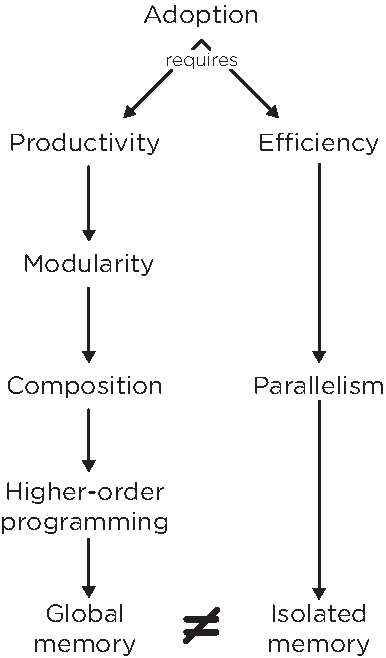
\includegraphics[width=0.35\textwidth]{../resources/insights.pdf}
}

This chapter concludes on the similar ground than the 1972 paper from D. Parnas \cite{Parnas1972}.
Productivity requires modularity through encapsulation and composition.
It requires higher-order programming which relies on a global memory abstraction as explained in section \ref{chapter3:software-productivity:efficiency-limitations}.
Whereas efficiency requires a balance between fine-grain level shared state with synchronization and coarse-grain level independence with message-passing.
This discontinuity between fine-grain level and coarse-grain level avoids the global memory abstraction, hence productivity.
The absence of a global memory abstraction reserves efficient platforms for an elite of developers.
No platform can support simultaneously productivity and efficiency.
Nonetheless, a platforms needs to be adopted both by the industry and the community to be sustainable.
D. Parnas then suggested the use of compilation techniques to bridge the gap between these two extremes.

However, more than this problem of immediate incompatibility, the problem holds on the evolution of the implementation.
No platform is able to follow a project from the early beginning until the industrial maturation of the project.
All the platforms tends to be stuck in a compromise between these two goals, and cannot follow the evolution required for this compromise.
These compromises are rigidly defined, while the need of the application is constantly evolving.
They lack the possibility to follow the organic evolution of a project.
Therefore, a project needs to change platform to change its priority, which leads to economical consequences.

To avoid these consequences, platforms would need to support productivity to allow the community to experiment, and organically start projects.
And then continuously shift toward efficiency as the project evolves, and requires it.
This thesis now explores this possibility.

%-----------------------------------------------------------------------------%
                                    \endinput
%-----------------------------------------------------------------------------%


Some links I NEED to put :
--------------------------

http://calculist.org/blog/2011/12/14/why-coroutines-wont-work-on-the-web/

Albert Cohen
https://scholar.google.com/citations?user=MkKZKAMAAAAJ&hl=en

+ Paul Feautrier (Tutor of A. Cohen)


Similar problem :
http://2015.splashcon.org/event/splash2015-splash-i-lindsey-kuper-talk
http://www.cs.indiana.edu/~lkuper/papers/lindsey-kuper-dissertation.pdf

PJS was abandoned :
https://groups.google.com/forum/#!topic/mozilla.dev.tech.js-engine/H-YEsejE6DA
https://bugzilla.mozilla.org/show_bug.cgi?id=1117724

See parallel JS for further work (maybe) :
http://smallcultfollowing.com/babysteps/blog/2014/04/24/parallel-pipelines-for-js/

Some chunks I might find useful later :
---------------------------------------

A good example of declarative sentence in everyday world : in case of fire, 
the elevators don't work -> you understand that you need to take the stairs.